\chapter{Multivariable Integral} \label{mi:chapter}


%%%%%%%%%%%%%%%%%%%%%%%%%%%%%%%%%%%%%%%%%%%%%%%%%%%%%%%%%%%%%%%%%%%%%%%%%%%%%%

\section{Riemann integral over rectangles}
\label{sec:rirect}

\sectionnotes{2--3 lectures}

As in \chapterref{int:chapter}, we define the Riemann integral using the Darboux
upper and lower integrals.  The ideas in this section are very similar to
integration in one dimension.  The complication is mostly notational.
The differences between one and several dimensions will grow more pronounced
in the sections following.

\subsection{Rectangles and partitions}

\begin{defn}
Let $(a_1,a_2,\ldots,a_n)$ and
$(b_1,b_2,\ldots,b_n)$ be such that $a_k \leq b_k$ for all $k$.
A set of the form
$[a_1,b_1] \times
[a_2,b_2] \times \cdots \times
[a_n,b_n]$ is called a \emph{\myindex{closed rectangle}}\index{rectangle}.
In this setting it is sometimes useful to allow $a_k = b_k$, in which case we 
think of $[a_k,b_k] = \{ a_k \}$ as usual.
If $a_k < b_k$ for all $k$, then a set of the form
$(a_1,b_1) \times
(a_2,b_2) \times \cdots \times
(a_n,b_n)$ is called an \emph{\myindex{open rectangle}}.

For an open or closed rectangle
$R := [a_1,b_1] \times
[a_2,b_2] \times \cdots \times
[a_n,b_n] \subset \R^n$
or
$R := (a_1,b_1) \times
(a_2,b_2) \times \cdots \times
(a_n,b_n) \subset \R^n$,
we define the
\emph{$n$-dimensional volume}%
\index{n-dimensional volume@$n$-dimensional volume!rectangles}%
\index{volume of rectangles} by
\glsadd{not:ndimvolume}
\begin{equation*}
V(R) :=
(b_1-a_1)
(b_2-a_2)
\cdots
(b_n-a_n) .
\end{equation*}

A \emph{\myindex{partition}} $P$ of the closed rectangle
$R = [a_1,b_1] \times
[a_2,b_2] \times \cdots \times
[a_n,b_n]$
is
a finite set of 
partitions $P_1,P_2,\ldots,P_n$ of the intervals
$[a_1,b_1], [a_2,b_2],\ldots, [a_n,b_n]$.
We write $P=(P_1,P_2,\ldots,P_n)$.
That is, for every $k$ there is an integer $\ell_k$ and the finite set
of numbers
$P_k = \{ x_{k,0},x_{k,1},x_{k,2},\ldots,x_{k,\ell_k} \}$ such that
\begin{equation*}
a_k = x_{k,0} < x_{k,1} < x_{k,2} < \cdots < x_{k,{\ell_k}-1} < x_{k,\ell_k} = b_k .
\end{equation*}
Picking a set of $n$ integers $j_1,j_2,\ldots,j_n$ where
$j_k \in \{ 1,2,\ldots,\ell_k \}$ we get
the
\emph{\myindex{subrectangle}}
\begin{equation*}
[x_{1,j_1-1}~,~ x_{1,j_1}]
\times
[x_{2,j_2-1}~,~ x_{2,j_2}]
\times
\cdots
\times
[x_{n,j_n-1}~,~ x_{n,j_n}] .
\end{equation*}
For simplicity, we order the subrectangles somehow and
we say $\{R_1,R_2,\ldots,R_N\}$ are the subrectangles corresponding
to the partition $P$ of $R$.  More simply, we say they are the subrectangles of
$P$.
In other words, we subdivided the original rectangle into many smaller
subrectangles.  See \figureref{mv:figrect}.  It is not difficult to see that
these subrectangles cover our original $R$, and their
volume sums to that of $R$.  That is,
\begin{equation*}
R= \bigcup_{j=1}^N R_j , \qquad \text{and} \qquad
V(R) = \sum_{j=1}^N V(R_j).
\end{equation*}

\begin{myfigureht}
\subimport*{figures/}{figrect.pdf_t}
\caption{Example partition of a rectangle in $\R^2$.  The order of the
subrectangles is not important.\label{mv:figrect}}
\end{myfigureht}

When
\begin{equation*}
R_k = [x_{1,j_1-1}~,~ x_{1,j_1}]
\times
[x_{2,j_2-1}~,~ x_{2,j_2}]
\times
\cdots
\times
[x_{n,j_n-1}~,~ x_{n,j_n}] ,
\end{equation*}
then
\begin{equation*}
V(R_k) = 
\Delta x_{1,j_1}
\Delta x_{2,j_2}
\cdots
\Delta x_{n,j_n}
=
(x_{1,j_1}-x_{1,j_1-1})
(x_{2,j_2}-x_{2,j_2-1})
\cdots
(x_{n,j_n}-x_{n,j_n-1}) .
\end{equation*}

Let $R \subset \R^n$ be a closed rectangle and
let $f \colon R \to \R$ be a bounded function.  Let $P$ be a partition of
$R$ and suppose that there are $N$ subrectangles $R_1,R_2,\ldots,R_N$.
Define
\glsadd{not:lowerdarbouxsum}
\glsadd{not:upperdarbouxsum}
\begin{align*}
& m_i := \inf \{ f(x) : x \in R_i \} , \\
& M_i := \sup \{ f(x) : x \in R_i \} , \\
& L(P,f) :=
\sum_{i=1}^N m_i V(R_i) , \\
& U(P,f) :=
\sum_{i=1}^N M_i V(R_i) .
\end{align*}
We call $L(P,f)$ the \emph{\myindex{lower Darboux sum}} and
$U(P,f)$ the \emph{\myindex{upper Darboux sum}}\index{Darboux sum}.
\end{defn}

The indexing in the definition may be complicated, but fortunately we generally
do not need to go back directly to the definition often.
We start proving facts about the Darboux sums analogous to the one-variable
results.

\begin{prop} \label{mv:sumulbound:prop}
Suppose $R \subset \R^n$ is a closed rectangle
and $f \colon R \to \R$ is a bounded function.  Let $m, M \in \R$ be 
such that for all $x \in R$ we have $m \leq f(x) \leq M$.  For any partition
$P$ of $R$
we have
\begin{equation*}
m \, V(R) \leq
L(P,f) \leq U(P,f)
\leq M\, V(R) .
\end{equation*}
\end{prop}

\begin{proof}
Let $P$ be a partition.  Then for all $i$ we have
$m \leq m_i$ and $M_i \leq M$.  Also $m_i \leq M_i$ for all $i$.  Finally
$\sum_{i=1}^N V(R_i) = V(R)$.  Therefore,
\begin{multline*}
m \, V(R) =
m \left( \sum_{i=1}^N V(R_i) \right)
=
\sum_{i=1}^N m \, V(R_i)
\leq
\sum_{i=1}^N m_i \, V(R_i)
\leq
\\
\leq
\sum_{i=1}^N M_i \, V(R_i)
\leq
\sum_{i=1}^N M \,V(R_i)
=
M \left( \sum_{i=1}^N V(R_i) \right)
=
M \,V(R) .  \qedhere
\end{multline*}
\end{proof}

\subsection{Upper and lower integrals}

By \propref{mv:sumulbound:prop} the set of upper and lower Darboux sums are bounded sets and we can take
their infima and suprema.  As before, we now make the following definition.

\begin{defn}
If $f \colon R \to \R$ is a bounded function on a closed rectangle $R \subset
\R^n$.
Define
\glsadd{not:lowerdarbouxR}
\glsadd{not:upperdarbouxR}
\begin{equation*}
\underline{\int_R} f
:= \sup \, \bigl\{ L(P,f) : P \text{ a partition of $R$} \bigr\} , 
\qquad
\overline{\int_R} f
:= \inf \, \bigl\{ U(P,f) : P \text{ a partition of $R$} \bigr\} .
\end{equation*}
We call $\underline{\int}$ the
\emph{\myindex{lower Darboux integral}}\index{Darboux integral} and
$\overline{\int}$ the \emph{\myindex{upper Darboux integral}}.
\end{defn}

As in one dimension we have refinements of partitions.

\begin{defn}
Let $R \subset \R^n$ be a closed rectangle.
Let $P = ( P_1, P_2, \ldots, P_n )$
and $\widetilde{P} = ( \widetilde{P}_1, \widetilde{P}_2, \ldots, \widetilde{P}_n )$
be partitions of $R$.  We say $\widetilde{P}$ a
\emph{refinement}\index{refinement of a partition} of $P$
if, as sets, $P_k \subset \widetilde{P}_k$ for all $k = 1,2,\ldots,n$.
\end{defn}

It is not difficult to see that if $\widetilde{P}$ is a refinement of $P$,
then subrectangles of $P$ are unions of subrectangles of $\widetilde{P}$.
Simply put, in a refinement we take the subrectangles of $P$,
and we cut them into smaller subrectangles.  See \figureref{mv:figrectpart}.

\begin{myfigureht}
\subimport*{figures/}{figrectpart.pdf_t}
\caption{Example refinement of a partition.  New ``cuts'' are marked in
dashed lines.  Do note that the exact order of the new subrectangles does not
matter.\label{mv:figrectpart}}
\end{myfigureht}

\begin{prop} \label{mv:prop:refinement}
Suppose $R \subset \R^n$ is a closed rectangle, $P$ is a partition of $R$
and $\widetilde{P}$ is a refinement of $P$.
If $f \colon R \to \R$ be a bounded function,
then
\begin{equation*}
L(P,f) \leq L(\widetilde{P},f) 
\qquad \text{and} \qquad
U(\widetilde{P},f) \leq U(P,f) .
\end{equation*}
\end{prop}

\begin{proof}
We prove the first inequality, the second follows similarly.
Let $R_1,R_2,\ldots,R_N$ be the subrectangles of $P$
and
$\widetilde{R}_1,\widetilde{R}_2,\ldots,\widetilde{R}_{\widetilde{N}}$ be the
subrectangles of
$\widetilde{R}$.
Let $I_k$ be the set of all indices $j$ such that $\widetilde{R}_j \subset R_k$.
For example, in figures \ref{mv:figrect} and
\ref{mv:figrectpart}, $I_4 = \{ 6, 7, 8, 9 \}$ as
$R_4 =
\widetilde{R}_6 \cup \widetilde{R}_7 \cup
\widetilde{R}_8 \cup \widetilde{R}_9$.
Then,
\begin{equation*}
R_k = \bigcup_{j \in I_k} \widetilde{R}_j,
\qquad
V(R_k) = \sum_{j \in I_k} V(\widetilde{R}_j).
\end{equation*}

Let $m_j := \inf \{ f(x) : x \in R_j \}$, and
$\widetilde{m}_j := \inf \{ f(x) : \in \widetilde{R}_j \}$ as usual.
If $j \in I_k$, then $m_k \leq \widetilde{m}_j$.  Then
\begin{equation*}
L(P,f) =
\sum_{k=1}^N m_k V(R_k)
=
\sum_{k=1}^N \sum_{j\in I_k} m_k V(\widetilde{R}_j)
\leq
\sum_{k=1}^N \sum_{j\in I_k} \widetilde{m}_j V(\widetilde{R}_j)
=
\sum_{j=1}^{\widetilde{N}} \widetilde{m}_j V(\widetilde{R}_j) = L(\widetilde{P},f) . \qedhere
\end{equation*}
\end{proof}

The key point of this next proposition is that
the lower Darboux integral is less than or equal to the upper Darboux
integral.

\begin{prop} \label{mv:intulbound:prop}
Let $R \subset \R^n$ be a closed rectangle and
$f \colon R \to \R$ a bounded function.  Let $m, M \in \R$ be 
such that for all $x \in R$ we have $m \leq f(x) \leq M$.  Then
\begin{equation}
\label{mv:intulbound:eq}
m \, V(R) \leq
\underline{\int_R} f \leq \overline{\int_R} f
\leq M \, V(R).
\end{equation}
\end{prop}

\begin{proof}
For any partition $P$, via \propref{mv:sumulbound:prop},
\begin{equation*}
mV(R) \leq L(P,f) \leq U(P,f) \leq M\,V(R).
\end{equation*}
Taking supremum of $L(P,f)$ and infimum of $U(P,f)$ over all $P$,
we obtain the first and the last inequality in
\eqref{mv:intulbound:eq}.

The key inequality in
\eqref{mv:intulbound:eq}
is the middle one.
Let $P=(P_1,P_2,\ldots,P_n)$ and
$Q=(Q_1,Q_2,\ldots,Q_n)$
be partitions of $R$.  Define 
$\widetilde{P} = ( \widetilde{P}_1,\widetilde{P}_2,\ldots,\widetilde{P}_n )$
by letting
$\widetilde{P}_k := P_k \cup Q_k$.
Then $\widetilde{P}$ is a partition of $R$ as can easily be checked,
and $\widetilde{P}$ is a refinement of $P$ and a refinement of $Q$.
By \propref{mv:prop:refinement},
$L(P,f) \leq L(\widetilde{P},f)$ and
$U(\widetilde{P},f) \leq U(Q,f)$.  Therefore,
\begin{equation*}
L(P,f) \leq L(\widetilde{P},f) \leq U(\widetilde{P},f) \leq U(Q,f) .
\end{equation*}
In other words, for two arbitrary partitions $P$ and $Q$ we have
$L(P,f) \leq U(Q,f)$.  
Via \volIref{Proposition~1.2.7 from volume I}, %\propref{infsupineq:prop}
we obtain
\begin{equation*}
\sup \, \bigl\{ L(P,f) : \text{$P$ a partition of $R$} \bigl\}
\leq
\inf \, \bigl\{ U(P,f) : \text{$P$ a partition of $R$} \bigl\} .
\end{equation*}
In other words $\underline{\int_R} f \leq \overline{\int_R} f$.
\end{proof}

\subsection{The Riemann integral}

We have all we need to
define the Riemann integral in $n$-dimensions over rectangles.
Again, the Riemann
integral is only defined on a certain class of functions, called the
Riemann integrable functions.

\begin{defn}
Let $R \subset \R^n$ be a closed rectangle.
Let $f \colon R \to \R$ be a bounded function such that
\begin{equation*}
\underline{\int_R} f(x)~dx = \overline{\int_R} f(x)~dx .
\end{equation*}
Then $f$ is said to be \emph{\myindex{Riemann integrable}},
and we sometimes say simply \emph{\myindex{integrable}}.
The set of Riemann integrable functions on $R$ is denoted
by $\sR(R)$.\glsadd{not:integrablefuncR}  When $f \in \sR(R)$ we define
the \emph{\myindex{Riemann integral}}
\glsadd{not:riemannintR}
\begin{equation*}
\int_R f := 
\underline{\int_R} f = \overline{\int_R} f .
\end{equation*}
\end{defn}

When the variable $x \in \R^n$ needs to be emphasized we write
\begin{equation*}
\int_R f(x)~dx,
\qquad
\int_R f(x_1,\ldots,x_n)~dx_1 \cdots dx_n,
\qquad
\text{or}
\qquad
\int_R f(x)~dV .
\end{equation*}
If $R \subset \R^2$, then often instead of volume we say area, and hence
write
\begin{equation*}
\int_R f(x)~dA .
\end{equation*}

\propref{mv:intulbound:prop} implies immediately the following
proposition.

\begin{prop} \label{mv:intbound:prop}
Let $f \colon R \to \R$ be a Riemann integrable function
on a closed rectangle $R \subset \R^n$.
Let $m, M \in \R$ be 
such that $m \leq f(x) \leq M$ for all $x \in R$.  Then
\begin{equation*}
m V(R) \leq
\int_{R} f
\leq M \, V(R) .
\end{equation*}
\end{prop}

\begin{example}
A constant function is Riemann integrable.  Suppose
$f(x) = c$ for all $x$ on $R$.  Then
\begin{equation*}
c V(R) \leq \underline{\int_R} f \leq \overline{\int_R} f \leq cV(R) .
\end{equation*}
So $f$ is integrable, and furthermore $\int_R f = cV(R)$.
\end{example}

The proofs of linearity and monotonicity are almost completely identical as
the proofs from one variable.  We therefore leave it as an exercise to prove
the next two propositions.

\begin{samepage}
\begin{prop}[Linearity] \label{mv:intlinearity:prop}
\index{linearity of the integral}
Let $R \subset \R^n$ be a closed rectangle and let
$f$ and $g$ be in $\sR(R)$ and $\alpha \in \R$.
\begin{enumerate}[(i)]
\item $\alpha f$ is in $\sR(R)$ and
\begin{equation*}
\int_R \alpha f = \alpha \int_R f .
\end{equation*}
\item $f+g$ is in $\sR(R)$ and
\begin{equation*}
\int_R (f+g) = 
\int_R f
+
\int_R g .
\end{equation*}
\end{enumerate}
\end{prop}
\end{samepage}

\begin{prop}[Monotonicity]
\index{monotonicity of the integral}
Let $R \subset \R^n$ be a closed rectangle, let
$f$ and $g$ be in $\sR(R)$, and suppose $f(x) \leq g(x)$
for all $x \in R$.  Then
\begin{equation*}
\int_R f 
\leq
\int_R g .
\end{equation*}
\end{prop}

Checking for integrability using the definition often involves the following
technique, as in the single variable case.

\begin{prop} \label{mv:prop:upperlowerepsilon}
Let $R \subset \R^n$ be a closed rectangle and
$f \colon R \to \R$ a bounded function.
Then $f \in \sR(R)$ if and only if
for every $\epsilon > 0$, there exists a partition $P$ of $R$
such that
\begin{equation*}
U(P,f) - L(P,f) < \epsilon .
\end{equation*}
\end{prop}

\begin{proof}
First, if $f$ is integrable, then clearly the supremum of $L(P,f)$ and
infimum of $U(P,f)$ must be equal and hence the
infimum of $U(P,f)-L(P,f)$ is zero.  Therefore for
every $\epsilon > 0$ there must be some partition $P$ such that 
$U(P,f) - L(P,f) < \epsilon$.

For the other direction, given an $\epsilon > 0$ find $P$ such that
$U(P,f) - L(P,f) < \epsilon$.
\begin{equation*}
\overline{\int_R} f - 
\underline{\int_R} f 
\leq
U(P,f) - L(P,f)
< \epsilon .
\end{equation*}
As $\overline{\int_R} f \geq \underline{\int_R} f$ and the above holds for
every $\epsilon > 0$, we conclude 
$\overline{\int_R} f = \underline{\int_R} f$ and $f \in \sR(R)$.
\end{proof}

For simplicity if $f \colon S \to \R$ is a function and $R \subset S$
is a closed rectangle, then if the restriction $f|_R$ is integrable we
say $f$ is integrable on $R$, or $f \in \sR(R)$ and we
write
\begin{equation*}
\int_R f := \int_R f|_R .
\end{equation*}

\begin{prop} \label{mv:prop:integralsmallerset}
For a closed rectangle $S \subset \R^n$,
if $f \colon S \to \R$ is integrable and $R \subset S$
is a closed rectangle, then $f$ is integrable over $R$.
\end{prop}

\begin{proof}
Given $\epsilon > 0$, we find a partition $P$ of $S$ such that
$U(P,f)-L(P,f) < \epsilon$.  By making a refinement of $P$
if necessary,
we assume that the endpoints of $R$ are in $P$.  In other words,
$R$ is a union of subrectangles of $P$.  The subrectangles of $P$
divide into two collections, ones that are subsets of $R$
and ones whose intersection with the interior of $R$ is empty.
Suppose $R_1,R_2\ldots,R_K$ are the subrectangles that
are subsets of $R$ and let $R_{K+1},\ldots, R_N$ be the rest.
Let $\widetilde{P}$ be the partition of $R$ composed of 
those subrectangles of $P$ contained in $R$.
Using the same notation as before,
\begin{equation*}
\begin{split}
\epsilon & > 
U(P,f)-L(P,f)
=
\sum_{k=1}^K (M_k-m_k) V(R_k)
+
\sum_{k=K+1}^N (M_k-m_k) V(R_k)
\\
&
\geq
\sum_{k=1}^K (M_k-m_k) V(R_k)
=
U(\widetilde{P},f|_R)-L(\widetilde{P},f|_R) .
\end{split}
\end{equation*}
Therefore, $f|_R$ is integrable.
\end{proof}

\subsection{Integrals of continuous functions}

Although later we will prove a much more general result, it is useful to start
with integrability of continuous functions.
First we wish to measure the fineness of partitions.  In one variable we
measured the length of a subinterval, in several variables, we similarly
measure the sides of a subrectangle.
We say a rectangle $R = [a_1,b_1] \times
[a_2,b_2] \times \cdots \times
[a_n,b_n]$ has \emph{longest side at most $\alpha$}\index{longest side} if
$b_k-a_k \leq \alpha$ for all $k=1,2,\ldots,n$.

\begin{prop} \label{prop:diameterrectangle}
If a rectangle $R \subset \R^n$ has longest side at most $\alpha$.  Then
for any $x,y \in R$,
\begin{equation*}
\snorm{x-y} \leq \sqrt{n} \, \alpha .
\end{equation*}
\end{prop}

\begin{proof}
\begin{equation*}
\begin{split}
\snorm{x-y} 
& =
\sqrt{
{(x_1-y_1)}^2
+
{(x_2-y_2)}^2
+ \cdots +
{(x_n-y_n)}^2
}
\\
& \leq
\sqrt{
{(b_1-a_1)}^2
+
{(b_2-a_2)}^2
+ \cdots +
{(b_n-a_n)}^2
}
\\
& \leq
\sqrt{
{\alpha}^2
+
{\alpha}^2
+ \cdots +
{\alpha}^2
}
=
\sqrt{n} \, \alpha .  \qedhere
\end{split}
\end{equation*}
\end{proof}


\begin{thm} \label{mv:thm:contintrect}
Let $R \subset \R^n$ be a closed rectangle and
$f \colon R \to \R$ a continuous function,
then $f \in \sR(R)$.
\end{thm}

\begin{proof}
The proof is analogous to the one variable proof with some complications.
The set $R$ is a closed and bounded subset of $\R^n$, and hence compact.  So
$f$ is not just continuous, but in fact uniformly continuous 
by \volIref{Theorem 7.5.11 from volume I}.
Let $\epsilon > 0$ be given.  Find a $\delta > 0$ such that
$\snorm{x-y} < \delta$ implies $\sabs{f(x)-f(y)} < \frac{\epsilon}{V(R)}$.

Let $P$ be a partition of $R$, such that longest side of any subrectangle
is strictly less than $\frac{\delta}{\sqrt{n}}$.
If $x, y \in R_k$ for some subrectangle $R_k$ of $P$ we have,
by the proposition above,
$\snorm{x-y} < \sqrt{n} \frac{\delta}{\sqrt{n}} = \delta$.  Therefore
\begin{equation*}
f(x)-f(y) \leq \sabs{f(x)-f(y)} < \frac{\epsilon}{V(R)} .
\end{equation*}
As $f$ is continuous on $R_k$, it attains a maximum and a minimum
on this subrectangle.
Let $x$ be a point where $f$ attains the maximum and $y$ be a point
where $f$ attains the minimum.  Then $f(x) = M_k$
and $f(y) = m_k$ in the notation from the definition of the integral.
Therefore,
\begin{equation*}
M_i-m_i = f(x)-f(y) < 
\frac{\epsilon}{V(R)} .
\end{equation*}
And so
\begin{equation*}
\begin{split}
U(P,f) - L(P,f)
& =
\left(
\sum_{k=1}^N
M_k V(R_k)
\right)
-
\left(
\sum_{k=1}^N
m_k V(R_k)
\right)
\\
& =
\sum_{k=1}^N
(M_k-m_k) V(R_k)
\\
& <
\frac{\epsilon}{V(R)}
\sum_{k=1}^N
V(R_k)
= \epsilon.
\end{split}
\end{equation*}
Via application of \propref{mv:prop:upperlowerepsilon} we find that $f \in
\sR(R)$.
%As $\epsilon > 0$ was arbitrary,
%\begin{equation*}
%\overline{\int_a^b} f = \underline{\int_a^b} f ,
%\end{equation*}
%and $f$ is Riemann integrable on $R$.
\end{proof}

\subsection{Integration of functions with compact support}

Let $U \subset \R^n$ be an open set and
$f \colon U \to \R$ be a function.  We say the
\emph{\myindex{support}} of $f$ is the set
\begin{equation*}
\operatorname{supp} (f) :=
\overline{
\{ x \in U : f(x) \not= 0 \}
} ,
\end{equation*}
where the closure is with respect to the subspace topology on $U$.
Recall that taking the closure with respect to the subspace
topology is the same as 
$\overline{
\{ x \in U : f(x) \not= 0 \}
} \cap U$, now taking the closure with respect to the ambient euclidean space
$\R^n$.
In particular,
$\operatorname{supp} (f) \subset U$.
That is, the support is the closure (in $U$) of the set of points where the
function is nonzero.  Its complement in $U$ is open.
If $x \in U$ and $x$ is not in the support of $f$,
then
$f$ is constantly zero in a whole neighborhood of $x$.

A function $f$ is said to have \emph{\myindex{compact support}}
if $\supp(f)$ is a compact set.

\begin{example}
The function $f \colon \R^2 \to \R$ defined by
\begin{equation*}
f(x,y) :=
\begin{cases}
-x{(x^2+y^2-1)}^2 & \text{if $\sqrt{x^2+y^2} \leq 1$}, \\
0 & \text{else},
\end{cases}
\end{equation*}
is continuous and its support is the closed unit disc
$C(0,1) = \bigl\{ (x,y) : \sqrt{x^2 + y^2} \leq 1 \bigr\}$, which is a compact set, so $f$ has compact support.
Do note that the function is zero on the entire $y$-axis
and on the unit circle, but
all points that lie in the closed unit disc are still within the support
as they are in the closure of points where $f$ is nonzero.
See \figureref{fig:compsup}.
\begin{myfigureht}
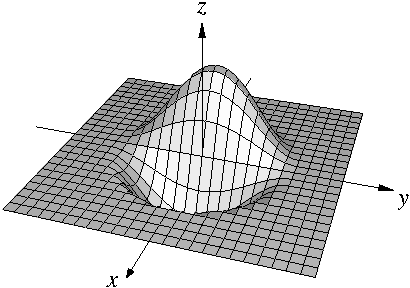
\includegraphics{figures/compsup}
\qquad
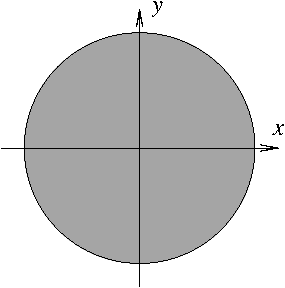
\includegraphics{figures/compsupsup}
\caption{Function with compact support (left), the support
is the closed unit disc (right).\label{fig:compsup}}
\end{myfigureht}
\end{example}

If $U \not= \R^n$, then you must be careful to
take the closure on the support in $U$.  Consider the following
two examples.

\begin{example}
Consider the unit disc $B(0,1) \subset \R^2$.
The function $f \colon B(0,1) \to \R$ defined by
\begin{equation*}
f(x,y) :=
\begin{cases}
0 & \text{if $\sqrt{x^2+y^2} > \nicefrac{1}{2}$}, \\
\nicefrac{1}{2} - \sqrt{x^2+y^2} & \text{if $\sqrt{x^2+y^2} \leq \nicefrac{1}{2}$},
\end{cases}
\end{equation*}
is continuous on $B(0,1)$ and its support is the smaller closed ball
$C(0,\nicefrac{1}{2})$.  As that is a compact set, $f$ has compact support.

Similarly $g \colon B(0,1) \to \R$ defined by
\begin{equation*}
g(x,y) :=
\begin{cases}
0 & \text{if $x \leq 0$}, \\
x & \text{if $x > 0$},
\end{cases}
\end{equation*}
is continuous on $B(0,1)$, but its support is the set
$\{ (x,y) \in B(0,1) : x \geq 0 \}$.  In particular, $g$ is not compactly
supported.
\end{example}

We will mostly consider the case when $U=\R^n$.  In light of
\exerciseref{exercise:contcompactsupportRn}, which says any continuous
function with compact support on $U \subset \R^n$ can be extended to a
continuous function with compact support on $\R^n$,
this is not an oversimplification.

\begin{example}
On the other hand for the unit disc $B(0,1) \subset \R^2$,
the function continuous $f \colon B(0,1) \to \R$ defined by $f(x,y) :=
\sin\bigl(\frac{1}{1-x^2-y^2}\bigr)$, does not have compact support; as
$f$ is not constantly zero on neighborhood of any point in $B(0,1)$,
we know that the support is the entire disc $B(0,1)$.  The function clearly
does not extend as above to a continuous function.  In fact it is not
difficult to show that it cannot be extended in any way whatsoever to be
continuous on all of $\R^2$ (the boundary of the disc is the problem).
\end{example}

\begin{prop} \label{mv:prop:rectanglessupp}
Suppose $f \colon \R^n \to \R$ be a continuous function with compact support.
If $R$ and $S$ are closed rectangles such that
$\operatorname{supp}(f) \subset R$
and
$\operatorname{supp}(f) \subset S$, then
\begin{equation*}
\int_S f = \int_R f .
\end{equation*}
\end{prop}

\begin{proof}
As $f$ is continuous, it is automatically integrable on the rectangles $R$, $S$, and $R
\cap S$.
Then \exerciseref{mv:zerooutside} says
$\int_S f = \int_{S \cap R} f = \int_R f$.
\end{proof}

Because of this proposition, when $f \colon \R^n \to \R$ has compact support
and is integrable over a rectangle $R$ containing the support we write
\begin{equation*}
\int f := \int_R f \qquad \text{or} \qquad 
\int_{\R^n} f := \int_R f .
\end{equation*}
For example, if $f$ is continuous and of compact support, then
$\int_{\R^n} f$ exists.

\subsection{Exercises}

\begin{exercise} \label{exercise:contcompactsupportRn}
Suppose $U \subset \R^n$ is open and $f \colon U \to \R$ is continuous and
of compact support.  Show that the function $\widetilde{f} \colon \R^n \to \R$
\begin{equation*}
\widetilde{f}(x) :=
\begin{cases}
f(x) & \text{ if $x \in U$,} \\
0 & \text{ otherwise,}
\end{cases}
\end{equation*}
is continuous.
\end{exercise}


\begin{exercise}
Prove \propref{mv:intlinearity:prop}.
\end{exercise}


\begin{exercise}
Suppose $R$ is a rectangle with the length of one of the sides equal to 0.
For any bounded function $f$, show that $f \in \sR(R)$ and $\int_R f = 0$.
\end{exercise}

\begin{exercise} \label{mv:zerosiderectangle}
Suppose $R$ is a rectangle with the length of one of the sides equal to 0,
and suppose $S$ is a rectangle with $R \subset S$.  If $f$
is a bounded function such that $f(x) = 0$ for $x \in R \setminus S$, show
that $f \in \sR(R)$ and $\int_R f = 0$.
\end{exercise}

\begin{exercise}
Suppose $f\colon \R^n \to \R$ is such that
$f(x) := 0$ if $x\not= 0$ and $f(0) := 1$.  Show that $f$ is integrable
on $R := [-1,1] \times [-1,1] \times \cdots \times [-1,1]$ directly using the
definition, and find $\int_R f$.
\end{exercise}

\begin{exercise} \label{mv:zeroinside}
Suppose $R$ is a closed rectangle and $h \colon R \to \R$ is a bounded function
such that $h(x) = 0$ if $x \notin \partial R$ (the boundary of $R$).
Let $S$ be any closed rectangle.
Show that $h \in \sR(S)$ and
\begin{equation*}
\int_{S} h = 0 .
\end{equation*}
Hint: Write $h$ as a sum of functions as in \exerciseref{mv:zerosiderectangle}.
\end{exercise}

\begin{exercise} \label{mv:zerooutside}
Suppose $R$ and $R'$ are two closed rectangles with $R' \subset R$.  Suppose $f \colon R \to \R$ is in $\sR(R')$
and $f(x) = 0$ for $x \in R \setminus R'$.
Show that $f \in \sR(R)$ and
\begin{equation*}
\int_{R'} f = \int_R f .
\end{equation*}
Do this in the following steps.
\begin{enumerate}[a)]
\item
First do the proof assuming that furthermore $f(x) = 0$ whenever $x
\in \overline{R \setminus R'}$.
\item
Write $f(x) = g(x) + h(x)$ where $g(x) = 0$ whenever $x
\in \overline{R \setminus R'}$, and $h(x)$ is zero except perhaps on
$\partial R'$.
Then show $\int_R h = \int_{R'} h = 0$ (see \exerciseref{mv:zeroinside}).
\item
Show 
$\int_{R'} f = \int_R f$.
\end{enumerate}
\end{exercise}

\begin{exercise}
Suppose $R' \subset \R^n$ and $R'' \subset \R^n$ are two rectangles
such that $R = R' \cup R''$ is a rectangle, and $R' \cap R''$ is rectangle
with one of the sides having length 0 (that is $V(R' \cap R'') = 0$).
Let $f \colon R \to \R$ be a function such that $f \in \sR(R')$ and
$f \in \sR(R'')$.  Show that $f \in \sR(R)$ and
\begin{equation*}
\int_{R} f = \int_{R'} f + \int_{R''} f .
\end{equation*}
Hint: see previous exercise.
\end{exercise}

\begin{exercise}
Prove a stronger version of \propref{mv:prop:rectanglessupp}.
Suppose $f \colon \R^n \to \R$ be a function with compact support but not
necessarily continuous.
Prove that
if $R$ is a closed rectangle such that $\operatorname{supp}(f) \subset R$
and $f$ is integrable over $R$, then for any other closed rectangle
$S$ with $\operatorname{supp}(f) \subset S$,
the function $f$ is integrable over $S$ and
$\int_S f = \int_R f$.
Hint:~See \exerciseref{mv:zerooutside}.
\end{exercise}

\begin{exercise}
Suppose $R$ and $S$ are closed rectangles of $\R^n$.
Define $f \colon \R^n \to \R$ as $f(x) := 1$ if 
$x \in R$, and $f(x) := 0$ otherwise.  Prove $f$ is integrable over $S$
and compute $\int_S f$.  Hint: Consider $S \cap R$.
\end{exercise}

\begin{samepage}
\begin{exercise}
Let $R = [0,1] \times [0,1] \subset \R^2$.
\begin{enumerate}[a)]
\item
Suppose $f \colon R \to \R$ is defined by
\begin{equation*}
f(x,y) := 
\begin{cases}
1 & \text{ if $x = y$,} \\
0 & \text{ else.}
\end{cases}
\end{equation*}
Show that $f \in \sR(R)$ and compute $\int_R f$.
\item
Suppose $f \colon R \to \R$ is defined by
\begin{equation*}
f(x,y) := 
\begin{cases}
1 & \text{ if $x \in \Q$ or $y \in \Q$,} \\
0 & \text{ else.}
\end{cases}
\end{equation*}
Show that $f \notin \sR(R)$.
\end{enumerate}
\end{exercise}
\end{samepage}

\begin{exercise}
Suppose $R$ is a closed rectangle, and suppose $S_j$ are closed rectangles
such that $S_j \subset R$ and $S_j \subset S_{j+1}$ for all $j$.
Suppose $f \colon R \to \R$ is bounded and $f \in \sR(S_j)$ for all $j$.
Show that $f \in \sR(R)$ and
\begin{equation*}
\lim_{j\to\infty} \int_{S_j} f = \int_R f .
\end{equation*}
\end{exercise}

\begin{exercise}
Suppose $f\colon [-1,1] \times [-1,1] \to \R$ is a Riemann
integrable function such $f(x) = -f(-x)$.  Using the definition prove
\begin{equation*}
\int_{[-1,1] \times [-1,1]} f = 0 .
\end{equation*}
%Hint: You can add points to make the partition ``symmetric''.
\end{exercise}

%%%%%%%%%%%%%%%%%%%%%%%%%%%%%%%%%%%%%%%%%%%%%%%%%%%%%%%%%%%%%%%%%%%%%%%%%%%%%%

\sectionnewpage
\section{Iterated integrals and Fubini theorem}
\label{sec:iteratedints}

\sectionnotes{1--2 lectures}

The Riemann integral in several variables
is hard to compute from the definition.
For one-dimensional Riemann integral we have the fundamental
theorem of calculus
%(FIXME link?)
and we can compute many integrals without
having to appeal to the definition of the integral.
We will rewrite 
a Riemann integral in several variables into
several one-dimensional Riemann integrals
by iterating.  However, if $f \colon [0,1]^2 \to \R$ is a Riemann integrable
function, it is not immediately clear if the three expressions
\begin{equation*}
\int_{[0,1]^2} f ,
\qquad
\int_0^1 \int_0^1 f(x,y) ~ dx ~ dy ,
\qquad \text{and}
\qquad
\int_0^1 \int_0^1 f(x,y) ~ dy ~ dx
\end{equation*}
are equal, or if the last two are even well-defined.

\begin{example}
Define 
\begin{equation*}
f(x,y) := 
\begin{cases}
1 & \text{ if $x=\nicefrac{1}{2}$ and $y \in \Q$,} \\
0 & \text{ otherwise.}
\end{cases}
\end{equation*}
Then $f$ is Riemann integrable on $R := [0,1]^2$ and $\int_R f = 0$.
Furthermore, $\int_0^1 \int_0^1 f(x,y) ~ dx ~ dy = 0$.
However
\begin{equation*}
\int_0^1 f(\nicefrac{1}{2},y) ~ dy
\end{equation*}
does not exist, so we cannot even write $\int_0^1 \int_0^1 f(x,y) ~ dy ~ dx$.

Proof:
Let us start with integrability of $f$.  We simply take the partition
of $[0,1]^2$ where the partition in the $x$ direction is
$\{ 0, \nicefrac{1}{2}-\epsilon,
\nicefrac{1}{2}+\epsilon,1\}$ and in the $y$ direction $\{ 0, 1 \}$ .
The subrectangles of the partition are
\begin{equation*}
R_1 := [0,
\nicefrac{1}{2}-\epsilon] \times [0,1],
\qquad
R_2 := [\nicefrac{1}{2}-\epsilon,
\nicefrac{1}{2}+\epsilon] \times [0,1],
\qquad
R_3 := [\nicefrac{1}{2}+\epsilon,1] \times [0,1] .
\end{equation*}
We have $m_1 = M_1 = 0$, $m_2 =0$, $M_2 = 1$, and $m_3 = M_3 = 0$.
Therefore,
\begin{equation*}
L(P,f) = 
m_1 V(R_1)
+
m_2 V(R_2)
+
m_3 V(R_3)
=
0 (\nicefrac{1}{2}-\epsilon)
+
0 (2\epsilon)
+
0 (\nicefrac{1}{2}-\epsilon) = 0 ,
\end{equation*}
and
\begin{equation*}
U(P,f) = 
M_1 V(R_1)
+
M_2 V(R_2)
+
M_3 V(R_3)
=
0 (\nicefrac{1}{2}-\epsilon)
+
1 (2\epsilon)
+
0 (\nicefrac{1}{2}-\epsilon) = 2 \epsilon .
\end{equation*}
The upper and lower sum are arbitrarily close and the lower sum is always
zero, so the function is integrable and $\int_R f = 0$.

For any $y$, the function that takes $x$ to $f(x,y)$ is zero except
perhaps at a single point $x=\nicefrac{1}{2}$.  We know that such a
function is integrable and $\int_0^1 f(x,y) ~ dx = 0$.  Therefore,
$\int_0^1 \int_0^1 f(x,y) ~ dx ~ dy = 0$.

However if $x=\nicefrac{1}{2}$, the function that takes $y$ to
$f(\nicefrac{1}{2},y)$ is the nonintegrable function that is
1 on the rationals and 0 on the irrationals.
See \volIref{Example 5.1.4 from volume I}.
\end{example}

We will solve this problem of undefined inside integrals
by using the upper and lower integrals, which are always defined.

\medskip

We split the coordinates of $\R^{n+m}$ into two parts.  That is,
we write the coordinates on $\R^{n+m} = \R^n \times \R^m$ as
$(x,y)$ where $x \in \R^n$ and $y \in \R^m$.  For a function $f(x,y)$
we write
\begin{equation*}
f_x(y) := f(x,y)
\end{equation*}
when $x$ is fixed and we wish to speak of the function in terms of $y$.
We write
\begin{equation*}
f^y(x) := f(x,y)
\end{equation*}
when $y$ is fixed and we wish to speak of the function in terms of $x$.

\begin{thm}[Fubini version A%
\footnote{Named after the Italian mathematician
\href{http://en.wikipedia.org/wiki/Guido_Fubini}{Guido Fubini}
(1879--1943).}] \label{mv:fubinivA}
Let $R \times S \subset \R^n \times \R^m$ be a closed rectangle and
$f \colon R \times S \to \R$ be integrable.
The functions $g \colon R \to \R$ and $h \colon R \to \R$ defined by
\begin{equation*}
g(x) := \underline{\int_S} f_x \qquad
\text{and} \qquad
h(x) := \overline{\int_S} f_x 
\end{equation*}
are integrable over $R$ and
\begin{equation*}
\int_R g = \int_R h = \int_{R \times S} f .
\end{equation*}
\end{thm}

In other words
\begin{equation*}
\int_{R \times S} f
=
 \int_R \left(
 \underline{\int_S} f(x,y) ~ dy
\right) ~ dx
=
 \int_R \left(
 \overline{\int_S} f(x,y) ~ dy
\right) ~ dx .
\end{equation*}
If it turns out that $f_x$ is integrable for all $x$, for example when
$f$ is continuous, then we obtain the more familiar
\begin{equation*}
\int_{R \times S} f
=
 \int_R \int_S f(x,y) ~ dy ~ dx .
\end{equation*}

\begin{proof}
Any partition of $R \times S$ is a concatenation of a partition of $R$ and a
partition of $S$.  That is, write a partition of $R \times S$
as $(P,P') = (P_1,P_2,\ldots,P_n,P'_1,P'_2,\ldots,P'_m)$,
where
$P = (P_1,P_2,\ldots,P_n)$ and
$P' = (P'_1,P'_2,\ldots,P'_m)$ are partitions of $R$ and $S$ respectively.
%Let $P$ be a partition of $R$ and $P'$ be a partition of $S$.
Let
$R_1,R_2,\ldots,R_N$ be the subrectangles of $P$ and
$R'_1,R'_2,\ldots,R'_K$ be the subrectangles of $P'$.
%Then
%if we concatenate the two partitions as $(P,P')$, that is
%if $P = (P_1,P_2,\ldots,P_n)$ and
%$P' = (P'_1,P'_2,\ldots,P'_m)$, we write
%$(P,P') = (P_1,P_2,\ldots,P_n,P'_1,P'_2,\ldots,P'_m)$.
Then the subrectangles of $(P,P')$ are
$R_j \times R'_k$ where $1 \leq j \leq N$ and $1 \leq k \leq K$.

Let
\begin{equation*}
m_{j,k} :=
\inf_{(x,y) \in R_j \times R'_k} f(x,y) .
\end{equation*}
We notice that
$V(R_j \times R'_k) = V(R_j)V(R'_k)$ and hence
\begin{equation*}
L\bigl((P,P'),f\bigr) =
\sum_{j=1}^N
\sum_{k=1}^K
m_{j,k} \, V(R_j \times R'_k)
=
\sum_{j=1}^N
\left(
\sum_{k=1}^K
m_{j,k} \, V(R'_k) \right) V(R_j) .
\end{equation*}
If we let
\begin{equation*}
m_k(x) := \inf_{y \in R'_k} f(x,y) = \inf_{y \in R'_k} f_x(y) ,
\end{equation*}
then of course if $x \in R_j$, then $m_{j,k} \leq m_k(x)$.  Therefore
\begin{equation*}
\sum_{k=1}^K
m_{j,k} \, V(R'_k)
\leq \sum_{k=1}^K m_k(x) \, V(R'_k) = L(P',f_x) \leq
\underline{\int_S} f_x = g(x) .
\end{equation*}
As we have the inequality for all $x \in R_j$ we have
\begin{equation*}
\sum_{k=1}^K
m_{j,k} \, V(R'_k)
\leq \inf_{x \in R_j} g(x) .
\end{equation*}
We thus obtain
\begin{equation*}
L\bigl((P,P'),f\bigr) 
\leq
\sum_{j=1}^N
\left(
\inf_{x \in R_j} g(x)
\right) V(R_j) = L(P,g) .
\end{equation*}

Similarly $U\bigl((P,P'),f) \geq U(P,h)$, and the proof of this inequality is
left as an exercise.

Putting this together we have
\begin{equation*}
L\bigl((P,P'),f\bigr)
\leq
L(P,g) \leq
U(P,g) \leq
U(P,h) \leq
U\bigl((P,P'),f\bigr) .
\end{equation*}
And since $f$ is integrable, it must be that $g$ is integrable as
\begin{equation*}
U(P,g) - L(P,g)
\leq
U\bigl((P,P'),f\bigr) -
L\bigl((P,P'),f\bigr) ,
\end{equation*}
and we can make the right hand side arbitrarily small.
As for any partition we have 
$L\bigl((P,P'),f\bigr) \leq L(P,g) \leq U\bigl((P,P'),f\bigr)$ we must have
that $\int_R g = \int_{R \times S} f$.

Similarly we have
\begin{equation*}
L\bigl((P,P'),f\bigr)
\leq
L(P,g) \leq
L(P,h) \leq
U(P,h) \leq
U\bigl((P,P'),f\bigr) ,
\end{equation*}
and hence
\begin{equation*}
U(P,h) - L(P,h)
\leq
U\bigl((P,P'),f\bigr) -
L\bigl((P,P'),f\bigr) .
\end{equation*}
So if $f$ is integrable so is $h$, and
as $L\bigl((P,P'),f\bigr) \leq L(P,h) \leq U\bigl((P,P'),f\bigr)$ we must have
that $\int_R h = \int_{R \times S} f$.
\end{proof}

We can also do the iterated integration in opposite order.
The proof of this version is almost identical to version A
(or follows quickly from version A), and
we leave it as an exercise to the reader.

\begin{thm}[Fubini version B]\label{mv:fubinivB}
Let $R \times S \subset \R^n \times \R^m$ be a closed rectangle and
$f \colon R \times S \to \R$ be integrable.
The functions $g \colon S \to \R$ and $h \colon S \to \R$ defined by
\begin{equation*}
g(y) := \underline{\int_R} f^y \qquad
\text{and} \qquad
h(y) := \overline{\int_R} f^y 
\end{equation*}
are integrable over $S$ and
\begin{equation*}
\int_S g = \int_S h = \int_{R \times S} f .
\end{equation*}
\end{thm}

That is we also have
\begin{equation*}
\int_{R \times S} f
=
 \int_S \left(
 \underline{\int_R} f(x,y) ~ dx
\right) ~ dy
=
 \int_S \left(
 \overline{\int_R} f(x,y) ~ dx
\right) ~ dy .
\end{equation*}

Next suppose that $f_x$ and $f^y$ are integrable for simplicity.
For example, suppose that $f$ is continuous.  Then by
putting the two versions together we obtain the familiar
\begin{equation*}
\int_{R \times S} f
=
 \int_R 
 \int_S f(x,y) ~ dy ~ dx 
=
 \int_S 
 \int_R f(x,y) ~ dx ~ dy .
\end{equation*}

Often the Fubini theorem is stated in two dimensions
for a continuous function $f \colon R \to
\R$ on a rectangle $R = [a,b] \times [c,d]$.  Then the Fubini theorem
states that
\begin{equation*}
\int_R f = \int_a^b \int_c^d f(x,y) ~dy~dx
=
\int_c^d \int_a^b f(x,y) ~dx~dy .
\end{equation*}
And the Fubini theorem is commonly thought of as the theorem that allows us
to swap the order of iterated integrals.

Repeatedly applying Fubini theorem gets us the following
corollary:
Let $R := [a_1,b_1] \times [a_2,b_2] \times \cdots \times [a_n,b_n] \subset
\R^n$ be a closed rectangle and let
$f \colon R \to \R$ be continuous.  Then
\begin{equation*}
\int_R f = 
\int_{a_1}^{b_1}
\int_{a_2}^{b_2}
\cdots
\int_{a_n}^{b_n}
f(x_1,x_2,\ldots,x_n)
\,
dx_n
\,
dx_{n-1}
\cdots
dx_1 .
\end{equation*}

Clearly we can also switch the order of integration to any order we please.
We can also relax the continuity requirement by making sure that all the
intermediate functions are integrable, or by using upper or lower integrals.

\subsection{Exercises}

\begin{exercise}
Compute $\int_{0}^1 \int_{-1}^1 xe^{xy} ~ dx ~ dy$ in a simple way.
\end{exercise}

\begin{exercise}
Prove the assertion
$U\bigl((P,P'),f\bigr) \geq U(P,h)$ from the proof
of \thmref{mv:fubinivA}.
\end{exercise}

\begin{exercise}[Easy]
Prove \thmref{mv:fubinivB}.
\end{exercise}

\begin{exercise}
Let $R=[a,b] \times [c,d]$ and $f(x,y)$ is an integrable
function on $R$ such that
such that for any fixed $y$, the function that takes $x$ to $f(x,y)$
is zero except at finitely many points.  Show
\begin{equation*}
\int_R f = 0 .
\end{equation*}
\end{exercise}

\begin{exercise}
Let $R=[a,b] \times [c,d]$ and $f(x,y) := g(x)h(y)$ for two continuous
functions $g \colon [a,b] \to \R$ and
$h \colon [a,b] \to \R$.  Prove
\begin{equation*}
\int_R f = \left(\int_a^b g\right)\left(\int_c^d h\right) .
\end{equation*}
\end{exercise}

%\begin{exercise}
%Compute
%\begin{equation*}
%FIXME: this one doesn't work
%\int_0^1 \int_0^1 x e^{y^2 + x^2} ~ dy ~ dx
%\end{equation*}
%\end{exercise}

\begin{exercise}
Compute
\begin{equation*}
\int_0^1 \int_0^1 \frac{x^2-y^2}{{(x^2+y^2)}^2} ~ dx ~ dy
\qquad \text{and} \qquad
\int_0^1 \int_0^1 \frac{x^2-y^2}{{(x^2+y^2)}^2} ~ dy ~ dx .
\end{equation*}
You will need to interpret the integrals as improper, that
is, the limit of $\int_\epsilon^1$ as $\epsilon \to 0$.
\end{exercise}

\begin{exercise}
Suppose $f(x,y) := g(x)$ where $g \colon [a,b] \to \R$ is Riemann integrable.
Show that $f$ is Riemann integrable for any $R = [a,b] \times [c,d]$ and 
\begin{equation*}
\int_R f = (d-c) \int_a^b g .
\end{equation*}
\end{exercise}

\begin{exercise}
Define $f \colon [-1,1] \times [0,1] \to \R$ by
\begin{equation*}
f(x,y) :=
\begin{cases}
x & \text{if $y \in \Q$,} \\
0 & \text{else.} 
\end{cases}
\end{equation*}
\begin{enumerate}[a)]
\item
Show
$\int_0^1 \int_{-1}^1 f(x,y) ~ dx ~ dy$ exists, but
$\int_{-1}^1 \int_0^1 f(x,y) ~ dy ~ dx$ does not.
\item
Compute
$\int_{-1}^1 \overline{\int_0^1} f(x,y) ~ dy ~ dx$ and
$\int_{-1}^1 \underline{\int_0^1} f(x,y) ~ dy ~ dx$.
\item
Show $f$ is not Riemann integrable on $[-1,1] \times [0,1]$ (use
Fubini).
\end{enumerate}
\end{exercise}

\begin{exercise}
Define $f \colon [0,1] \times [0,1] \to \R$ by
\begin{equation*}
f(x,y) :=
\begin{cases}
\nicefrac{1}{q} & \text{if $x \in \Q$, $y \in \Q$, and $y=\nicefrac{p}{q}$ in lowest terms,} \\
0 & \text{else.} 
\end{cases}
\end{equation*}
\begin{enumerate}[a)]
\item
Show $f$ is Riemann integrable on $[0,1] \times [0,1]$.
\item
Find 
$\overline{\int_0^1} f(x,y) ~ dx$ and
$\underline{\int_0^1} f(x,y) ~ dx$ for all $y \in [0,1]$, and show they are unequal for all $y
\in \Q$.
\item
Show
$\int_0^1 \int_0^1 f(x,y) ~ dy ~ dx$ exists, but
   $\int_0^1 \int_0^1 f(x,y) ~ dx ~ dy$ does not.
\end{enumerate}
Note: By Fubini,
$\int_0^1 \overline{\int_0^1} f(x,y) ~ dy ~ dx$ and 
$\int_0^1 \underline{\int_0^1} f(x,y) ~ dy ~ dx$ do exist and equal the
integral of $f$ on $R$.
\end{exercise}

%%%%%%%%%%%%%%%%%%%%%%%%%%%%%%%%%%%%%%%%%%%%%%%%%%%%%%%%%%%%%%%%%%%%%%%%%%%%%%

\sectionnewpage
\section{Outer measure and null sets}
\label{sec:outermeasure}

\sectionnotes{2 lectures}

%\subsection{Content zero sets}
%
%\begin{defn}
%A set $S \subset \R^n$ is a \emph{\myindex{content zero set}}
%if for every $\epsilon > 0$
%there exist a finite set of open rectangles $R_1, R_2, \ldots, R_k$ such that
%\begin{equation*}
%S \subset R_1 \cup R_2 \cup \ldots R_k \qquad \text{and} \qquad
%V(R_1) + V(R_2) + \cdots + V(R_k) < \epsilon.
%\end{equation*}
%\end{defn}
%
%Obviously if $S$ is content zero and $S' \subset S$, then
%$S'$ is of content zero.  We can in fact use the same exact rectangles.
%
%\begin{example}
%A finite set is of content zero.
%
%\emph{Proof:}
%FIXME
%\end{example}
%
%\begin{example}
%An open rectangle is not of content zero.
%
%\emph{Proof:}
%FIXME
%\end{example}
%
%\begin{example}
%The set $\Q^n \subset \R^n$ is not of content zero.
%
%\emph{Proof:}
%FIXME
%\end{example}

\subsection{Outer measure and null sets}

%FIXME
%
%\begin{defn}
%Let $(a_1,a_2,\ldots,a_n)$ and
%$(b_1,b_2,\ldots,b_n)$ be such that $a_k < b_k$ for all $k$.
%A set of the form
%$(a_1,b_1) \times
%(a_2,b_2) \times \cdots \times
%(a_n,b_n)$ is called an \emph{\myindex{open rectangle}}
%
%For an open rectangle
%$R := (a_1,b_1) \times
%(a_2,b_2) \times \cdots \times
%(a_n,b_n) \subset \R^n$ we define the
%\emph{$n$-dimensional volume}%
%\index{$n$-dimensional volume of rectangles}%
%\index{volume of rectangles} by
%\begin{equation*}
%V(R) :=
%(b_1-a_1)
%(b_2-a_2)
%\cdots
%(b_n-a_n) .
%\end{equation*}
%\end{defn}
%
%FIXME

Before we characterize all Riemann integrable functions, we need to make
a slight detour.  We introduce a way of measuring the size of sets in $\R^n$.

\begin{defn}
Let 
$S \subset \R^n$ be a subset.  Define the \emph{\myindex{outer measure}}
of $S$ as
\glsadd{not:outermeasure}
\begin{equation*}
m^*(S)
:=
\inf\,
\sum_{j=1}^\infty V(R_j) ,
\end{equation*}
where the infimum is taken over all sequences
$\{ R_j \}$ of open rectangles such that
%\begin{equation*}
$S \subset \bigcup_{j=1}^\infty R_j$.
%\end{equation*}
In particular, $S$ is of \emph{\myindex{measure zero}} or
a \emph{\myindex{null set}} if $m^*(S) = 0$.
\end{defn}

The theory of measures on $\R^n$ is a very complicated subject.
We will only require measure-zero sets and so we focus on these.
The set $S$ is of measure zero if
for every $\epsilon > 0$
there exist a sequence of open rectangles $\{ R_j \}$ such that
\begin{equation} \label{mv:eq:nullR}
S \subset \bigcup_{j=1}^\infty R_j \qquad \text{and} \qquad
\sum_{j=1}^\infty V(R_j) < \epsilon.
\end{equation}
Furthermore, 
if $S$ is of measure zero and $S' \subset S$, then
$S'$ is of measure zero.  We can use the same exact rectangles.

It is sometimes more convenient to use balls instead of rectangles.
Furthermore, we can
choose balls no bigger than a fixed radius.
%  The proof of the following proposition is left
%as an exercise (see \exerciseref{mv:exercise:ballsnull}).

\begin{prop} \label{mv:prop:ballsnull}
Let $\delta > 0$ be given.
A set $S \subset \R^n$ is measure zero if and only if for every $\epsilon >
0$, there exists a sequence of open balls $\{ B_j \}$, where the radius of
$B_j$ is $r_j < \delta$ such that
\begin{equation*}
S \subset \bigcup_{j=1}^\infty B_j \qquad \text{and} \qquad
\sum_{j=1}^\infty r_j^n < \epsilon.
\end{equation*}
\end{prop}

Note that the ``volume'' of $B_j$ is proportional to $r_j^n$.

\begin{proof}
If $R$ is a (closed or open) cube (rectangle with all sides
equal) of side $s$, then $R$ is contained in a closed ball of radius
$\sqrt{n}\, s$ by \propref{prop:diameterrectangle}, and therefore
in an open ball of size $2 \sqrt{n}\, s$.

Let $s$ be a number that is less than the smallest side of $R$ and also
so that $2\sqrt{n} \, s < \delta$.
We claim $R$ is contained in
a union of closed cubes $C_1, C_2, \ldots, C_k$ of sides $s$ such that
\begin{equation*}
\sum_{j=1}^k V(C_j) \leq 2^n V(R) .
\end{equation*}
It is clearly true (without the $2^n$) if $R$ has sides that are
integer multiples of $s$.  So if a side is of length $(\ell+\alpha) s$, for
$\ell \in \N$ and $0 \leq \alpha < 1$, then
$(\ell+\alpha)s \leq 2\ell s$.  Increasing the side to $2\ell s$ we obtain a new larger
rectangle of volume at most $2^n$ times larger, but whose sides are
multiples of $s$.

So suppose that there exist $\{ R_j \}$ as in the definition such that
\eqref{mv:eq:nullR} is true.  As we have seen above, we can choose closed
cubes $\{ C_k \}$ with $C_k$ of side $s_k$ as above that cover all the rectangles $\{ R_j \}$
and so that
\begin{equation*}
\sum_{k=1}^\infty s_k^n =
\sum_{k=1}^\infty V(C_k) \leq
2^n \sum_{j=1}^\infty V(R_k)
< 2^n \epsilon.
\end{equation*}
Covering $C_k$ with balls $B_k$ of radius $r_k = 2\sqrt{n} \, s_k$ we obtain 
\begin{equation*}
\sum_{k=1}^\infty r_k^n <
2^{2n} n \epsilon .
\end{equation*}
And as $S \subset\bigcup_{j} R_j \subset \bigcup_{k} C_k \subset \bigcup_{k}
B_k$, we are finished.

Suppose we have the ball condition above for some $\epsilon > 0$.
Without loss of generality assume that all $r_j < 1$.
Each $B_j$ is contained a in a cube $R_j$ of side $2r_j$.
So $V(R_j) = {(2 r_j)}^n < 2^n r_j$.  Therefore 
\begin{equation*}
S \subset \bigcup_{j=1}^\infty R_j \qquad \text{and} \qquad
\sum_{j=1}^\infty V(R_j)
<
\sum_{j=1}^\infty 2^n r_j < 2^n \epsilon. \qedhere
\end{equation*}
\end{proof}

The definition of outer measure could have been done with open balls
as well, not just null sets.  We leave this generalization to the reader.

\subsection{Examples and basic properties}

\begin{example}
The set $\Q^n \subset \R^n$ of points with rational coordinates
is a set of measure zero.

\emph{Proof:}
The set $\Q^n$ is countable and therefore let us write it
as a sequence $q_1,q_2,\ldots$.  For each $q_j$ find an open rectangle
$R_j$ with $q_j \in R_j$ and $V(R_j) < \epsilon 2^{-j}$.  Then
\begin{equation*}
\Q^n \subset \bigcup_{j=1}^\infty R_j \qquad \text{and} \qquad
\sum_{j=1}^\infty V(R_j) <
\sum_{j=1}^\infty \epsilon 2^{-j} = \epsilon .
\end{equation*}
\end{example}

The example points to a more general result.

\begin{prop}
A countable union of measure zero sets is of measure zero.
\end{prop}

\begin{proof}
Suppose
\begin{equation*}
S = \bigcup_{j=1}^\infty S_j ,
\end{equation*}
where $S_j$ are all measure zero sets.  Let $\epsilon > 0$ be given.
For each $j$
there exists a sequence of open rectangles $\{ R_{j,k} \}_{k=1}^\infty$
such that
\begin{equation*}
S_j \subset \bigcup_{k=1}^\infty R_{j,k}
\end{equation*}
and 
\begin{equation*}
\sum_{k=1}^\infty V(R_{j,k}) < 2^{-j} \epsilon .
\end{equation*}
Then
\begin{equation*}
S \subset \bigcup_{j=1}^\infty \bigcup_{k=1}^\infty R_{j,k} .
\end{equation*}
As $V(R_{j,k})$ is always positive, the sum over all $j$ and $k$
can be done in any order.  In particular, it can be done as
\begin{equation*}
\sum_{j=1}^\infty \sum_{k=1}^\infty V(R_{j,k}) <
\sum_{j=1}^\infty 2^{-j} \epsilon = \epsilon . \qedhere
\end{equation*}
\end{proof}

The next example is not just interesting, it will be useful later.

\begin{example} \label{mv:example:planenull}
Let $P := \{ x \in \R^n : x_k = c \}$ for a fixed $k=1,2,\ldots,n$ and
a fixed constant $c \in \R$.  Then $P$ is of measure zero.

\emph{Proof:}
First fix $s$ and let us prove that
\begin{equation*}
P_s := \bigl\{ x \in \R^n : x_k = c, \sabs{x_j} \leq s \text{ for all
$j\not=k$} \bigr\}
\end{equation*}
is of measure zero.
Given any $\epsilon > 0$ define the open rectangle
\begin{equation*}
R := \bigl\{ x \in \R^n : c-\epsilon < x_k < c+\epsilon, \sabs{x_j} < s+1
\text{ for all $j\not=k$} \bigr\} .
\end{equation*}
It is clear that $P_s \subset R$.  Furthermore
\begin{equation*}
V(R) = 2\epsilon {\bigl(2(s+1)\bigr)}^{n-1} .
\end{equation*}
As $s$ is fixed, we can
make $V(R)$
arbitrarily small by
picking $\epsilon$ small enough.

Next we note that
\begin{equation*}
P = \bigcup_{j=1}^\infty P_j
\end{equation*}
and a countable union of measure zero sets is measure zero.
\end{example}

\begin{example}
If $a < b$, then $m^*\bigl([a,b]\bigr) = b-a$.

\emph{Proof:}
In the case of $\R$, open rectangles are open intervals.
Since $[a,b] \subset (a-\epsilon,b+\epsilon)$ for all $\epsilon > 0$.
Hence, $m^*\bigl([a,b]\bigr) \leq b-a$.

Let us prove the other inequality.
Suppose $\bigl\{ (a_j,b_j) \bigr\}$ are open intervals such that
\begin{equation*}
[a,b] \subset \bigcup_{j=1}^\infty (a_j,b_j) .
\end{equation*}
We wish to bound $\sum (b_j-a_j)$ from below.
Since $[a,b]$ is compact, then there are only finitely many open intervals
that still cover $[a,b]$.  As throwing out some of the intervals only makes the
sum smaller, we only need to take the finite number of intervals
still covering $[a,b]$.
If $(a_i,b_i) \subset (a_j,b_j)$, then we can throw out
$(a_i,b_i)$ as well.
Therefore we have
$[a,b] \subset \bigcup_{j=1}^k (a_j,b_j)$ for some $k$, and
we assume that the intervals are sorted such that $a_1 < a_2 < \cdots <
a_k$.  Note that since $(a_2,b_2)$ is not contained in $(a_1,b_1)$
we have that $a_1 < a_2 < b_1 < b_2$.  Similarly
$a_j < a_{j+1} < b_j < b_{j+1}$.  Furthermore, $a_1 < a$ and $b_k > b$.
Thus,
\begin{equation*}
m^*\bigl([a,b]\bigr) \geq
\sum_{j=1}^k (b_j-a_j)
\geq
\sum_{j=1}^{k-1} (a_{j+1}-a_j)
+
(b_k-a_k)
=
b_k-a_1 > b-a .
\end{equation*}
\end{example}

\begin{prop} \label{mv:prop:compactnull}
Suppose $E \subset \R^n$ is a compact set of measure zero.  Then for
every $\epsilon > 0$, there exist
finitely many open rectangles $R_1,R_2,\ldots,R_k$ such that
\begin{equation*}
E \subset R_1 \cup R_2 \cup \cdots \cup R_k
\qquad \text{and} \qquad
\sum_{j=1}^k V(R_j) < \epsilon.
\end{equation*}
Also for any $\delta > 0$,
there exist finitely many open balls $B_1,B_2,\ldots,B_k$ of radii
$r_1,r_2,\ldots,r_k < \delta$ such that
\begin{equation*}
E \subset B_1 \cup B_2 \cup \cdots \cup B_k
\qquad \text{and} \qquad
\sum_{j=1}^k r_j^n < \epsilon.
\end{equation*}
\end{prop}

\begin{proof}
Find a sequence of open rectangles $\{ R_j \}$ such that 
\begin{equation*}
E \subset \bigcup_{j=1}^\infty R_j
\qquad \text{and} \qquad
\sum_{j=1}^\infty V(R_j) < \epsilon.
\end{equation*}
By compactness, there are finitely
many of these rectangles that still contain $E$.  That is, there is some $k$ such
that
$E \subset R_1 \cup R_2 \cup \cdots \cup R_k$.  Hence
\begin{equation*}
\sum_{j=1}^k V(R_j) \leq
\sum_{j=1}^\infty V(R_j) < \epsilon.
\end{equation*}

The proof that we can choose balls instead of rectangles is left as an
exercise.
\end{proof}

\begin{example} \label{example:cantor}
So that the reader is not under the impression that there are only very few
measure zero sets and that these are simple,
let us give an uncountable, compact, measure zero subset in $[0,1]$.
For any $x \in [0,1]$ write the
representation in ternary notation
\begin{equation*}
x = \sum_{j=1}^\infty d_n 3^{-n} .
\end{equation*}
See \volIref{\S1.5 in volume I, in particular Exercise 1.5.4}.
Define the \emph{\myindex{Cantor set}} $C$ as
\begin{equation*}
C := \Bigl\{ x \in [0,1] : x = \sum_{j=1}^\infty d_n 3^{-n}, \text{ where $d_j =
0$ or $d_j = 2$ for all $j$} \Bigr\} .
\end{equation*}
That is, $x$ is in $C$ if it has a ternary expansion in only $0$'s and
$2$'s.  If $x$ has two expansions, as long as one of them does not have any
$1$'s, then $x$ is in $C$.
Define $C_0 := [0,1]$ and
\begin{equation*}
C_k := \Bigl\{ x \in [0,1] : x = \sum_{j=1}^\infty d_n 3^{-n}, \text{ where $d_j =
0$ or $d_j = 2$ for all $j=1,2,\ldots,k$} \Bigr\} .
\end{equation*}
Clearly,
\begin{equation*}
C = \bigcap_{k=1}^\infty C_k .
\end{equation*}

\pagebreak[2]
We leave as an exercise to prove that:
\begin{enumerate}[(i)]
\item Each $C_k$ is a finite union of closed intervals.  It is obtained by
taking $C_{k-1}$, and from each closed interval removing the ``middle
third''.
\item Therefore, each $C_k$ is closed.
\item Furthermore,
$m^*(C_k) =1 - \sum_{n=1}^k \frac{2^n}{3^{n+1}}$.
\item Hence,
$m^*(C) = 0$.
\item The set $C$ is in one to one correspondence with $[0,1]$, in other
words,
uncountable.
\end{enumerate}
\begin{myfigureht}
\subimport*{figures/}{cantorfig.pdf_t}
\caption{Cantor set construction.\label{fig:cantor}}
\end{myfigureht}
See \figureref{fig:cantor}.
\end{example}


\subsection{Images of null sets}

Before we look at images of measure zero sets, let us see what a
continuously differentiable function does to a ball.

\begin{lemma} \label{lemma:ballmapder}
Suppose $U \subset \R^n$ is an open set,
$B \subset U$ is an open or closed ball of radius at most $r$, $f \colon B \to \R^n$ is continuously
differentiable and suppose $\snorm{f'(x)} \leq M$ for all $x \in B$.
Then $f(B) \subset B'$, where $B'$ is a ball of radius at most $Mr$.
\end{lemma}

\begin{proof}
Without loss of generality assume $B$ is a closed ball.
The ball $B$ is convex, and hence via
\propref{mv:prop:convexlip},
that $\snorm{f(x)-f(y)} \leq M \snorm{x-y}$
for all $x,y$ in $B$.  In particular, suppose $B = C(y,r)$,
then $f(B) \subset C\bigl(f(y),M r \bigr)$.
\end{proof}

The image of a measure zero set using a continuous map is not necessarily
a measure zero set.  However if we assume the mapping is continuously
differentiable, then the mapping cannot ``stretch'' the set too much.
%The proposition does not require compactness, and this is left as an
%exercise.

\begin{prop} \label{prop:imagenull}
Suppose $U \subset \R^n$ is an open set and $f \colon U \to \R^n$
is a continuously differentiable mapping.  If $E \subset U$ is a 
measure zero set, then $f(E)$ is measure zero.
\end{prop}

\begin{proof}
We leave the proof for a general measure zero set as an exercise, and we
now prove the proposition for a compact measure zero set.  Therefore let us 
suppose $E$ is compact.

First let us replace $U$ by a smaller open set to make $\snorm{f'(x)}$ bounded.
At each point $x \in
E$ pick an open ball $B(x,r_x)$ such that the closed ball $C(x,r_x) \subset
U$.  By compactness we only need to take finitely
many points $x_1,x_2,\ldots,x_q$ to still cover $E$.  Define
\begin{equation*}
U' := \bigcup_{j=1}^q B(x_j,r_{x_j}), \qquad
K := \bigcup_{j=1}^q C(x_j,r_{x_j}).
\end{equation*}
We have $E \subset U' \subset K \subset U$.  The set $K$ is compact.
The function that takes $x$ to $\snorm{f'(x)}$ is continuous, and therefore
there exists an $M > 0$ such that $\snorm{f'(x)} \leq M$ for all $x \in K$.
So without loss of generality we may replace $U$ by $U'$ and from now on
suppose that $\snorm{f'(x)} \leq M$ for all $x \in U$.

At each point $x \in E$ pick a ball $B(x,\delta_x)$ of maximum radius 
so that $B(x,\delta_x) \subset U$.  Let $\delta = \inf_{x\in E} \delta_x$.
Take a sequence $\{ x_j \} \subset E$ so that $\delta_{x_j} \to \delta$.
As $E$ is compact, we can pick the sequence to be convergent to some $y \in
E$.  Once $\snorm{x_j-y} < \frac{\delta_y}{2}$, then
$\delta_{x_j} > \frac{\delta_y}{2}$ by the triangle inequality.
Therefore $\delta > 0$.

Given $\epsilon > 0$, there exist balls $B_1,B_2,\ldots,B_k$ of radii
$r_1,r_2,\ldots,r_k < \delta$ such that
\begin{equation*}
E \subset B_1 \cup B_2 \cup \cdots \cup B_k
\qquad \text{and} \qquad
\sum_{j=1}^k r_j^n < \epsilon.
\end{equation*}
Suppose $B_1', B_2', \ldots, B_k'$ are the balls of radius
$Mr_1, Mr_2, \ldots, Mr_k$ from
\lemmaref{lemma:ballmapder}, such that $f(B_j) \subset B_j'$ for all $j$.
\begin{equation*}
f(E) \subset f(B_1) \cup f(B_2) \cup \cdots \cup f(B_k)
\subset B_1' \cup B_2' \cup \cdots \cup B_k'
\qquad \text{and} \qquad
\sum_{j=1}^k Mr_j^n
%=
%M
%\sum_{j=1}^k Mr_j^n
 < M \epsilon. \qedhere
\end{equation*}
\end{proof}

\subsection{Exercises}

%FIXME:

%\begin{exercise} \label{mv:exercise:ballsnull}
%Prove \propref{mv:prop:ballsnull}.  Hint \propref{prop:diameterrectangle}
%for one direction.  For the other direction
%\end{exercise}

\begin{exercise}
Finish the proof of \propref{mv:prop:compactnull}, that is, show that you
can use balls instead of rectangles.
\end{exercise}

\begin{exercise}
If $A \subset B$, then $m^*(A) \leq m^*(B)$.
\end{exercise}

\begin{exercise}
Suppose $X \subset \R^n$ is a set such that for every $\epsilon > 0$
there exists a set $Y$ such that $X \subset Y$ and $m^*(Y) \leq \epsilon$.
Prove that $X$ is a measure zero set.
\end{exercise}

\begin{exercise}
Show that if $R \subset \R^n$ is a closed rectangle, then $m^*(R) = V(R)$.
\end{exercise}

\begin{exercise}
The closure of a measure zero set can be quite large.  Find an example
set $S \subset \R^n$ that is of measure zero, but whose closure
$\widebar{S} = \R^n$.
\end{exercise}

\begin{samepage}
\begin{exercise}
Prove the general case of  \propref{prop:imagenull} without using compactness:
\begin{enumerate}[a)]
\item
Mimic the proof to first prove that the proposition holds if $E$ is
\emph{\myindex{relatively compact}}; a set $E \subset U$ is relatively
compact if the closure of $E$ in the subspace topology on $U$ is compact,
or in other words if there exists a compact set $K$ with $K \subset U$
and $E \subset K$.\\
Hint: The bound on the size of the derivative still holds, but you need
to use countably many balls in the second part of the proof.
Be careful as the closure of $E$ need no
longer be measure zero.
\item
Now prove it for any null set $E$.\\
Hint: First show that $\{ x \in U : d(x,y) \geq
\nicefrac{1}{m} \text{ for all $y \notin U$ and } d(0,x) \leq m \}$ is a compact set for
any $m > 0$.
\end{enumerate}
\end{exercise}
\end{samepage}

\begin{exercise}
Let $U \subset \R^n$ be an open set
and let $f \colon U \to \R$ be a continuously differentiable function.
Let $G := \{ (x,y) \in U \times \R : y = f(x) \}$ be the graph of $f$.
Show that $f$ is of measure zero.
\end{exercise}

\begin{exercise}
Given a closed rectangle $R \subset \R^n$, show that for any $\epsilon > 0$
there exists a number $s > 0$ and finitely many open cubes $C_1,C_2,\ldots,C_k$
of side $s$ such that
$R \subset C_1 \cup C_2 \cup \cdots \cup C_k$
and
\begin{equation*}
\sum_{j=1}^k V(C_j) \leq V(R) + \epsilon .
\end{equation*}
\end{exercise}

\begin{exercise}
Show that there exists a number $k = k(n,r,\delta)$ depending only on $n$,
$r$ and $\delta$ such
the following holds.
Given $B(x,r) \subset \R^n$ and $\delta > 0$, there exist
$k$ open balls $B_1,B_2,\ldots,B_k$ of radius at most
$\delta$ such that $B(x,r) \subset B_1 \cup B_2 \cup \cdots \cup B_k$.
Note that you can find $k$ that really only depends on $n$ and the ratio
$\nicefrac{\delta}{r}$.
\end{exercise}

\begin{exercise}
Prove the statements of \exampleref{example:cantor}.  That is,
prove:
\begin{enumerate}[a)]
\item
Each $C_k$ is a finite union of closed intervals, and so $C$ is closed.
\item
$m^*(C_k) =1 - \sum_{n=1}^k \frac{2^n}{3^{n+1}}$.
\item
$m^*(C) = 0$.
\item
The set $C$ is in one to one correspondence with $[0,1]$.
\end{enumerate}
\end{exercise}


%%%%%%%%%%%%%%%%%%%%%%%%%%%%%%%%%%%%%%%%%%%%%%%%%%%%%%%%%%%%%%%%%%%%%%%%%%%%%%

\sectionnewpage
\section{The set of Riemann integrable functions }
\label{sec:riemannlebesgue}

\sectionnotes{1 lecture}

\subsection{Oscillation and continuity}

Let $S \subset \R^n$ be a set and $f \colon S \to \R$ a function.
Instead of just saying that $f$ is or is not continuous at
a point $x \in S$,
we need to be able to quantify how discontinuous $f$ is at a function is
at $x$.  For any $\delta > 0$ define the oscillation of 
$f$ on the $\delta$-ball in subspace topology that is
$B_S(x,\delta) = B_{\R^n}(x,\delta) \cap S$ as
\begin{equation*}
o(f,x,\delta) :=
{\sup_{y \in B_S(x,\delta)} f(y)}
-
{\inf_{y \in B_S(x,\delta)} f(y)}
= 
\sup_{y_1,y_2 \in B_S(x,\delta)} \bigl(f(y_1)-f(y_2)\bigr) .
\end{equation*}
That is, $o(f,x,\delta)$ is the length of the smallest interval
that contains the image $f\bigl(B_S(x,\delta)\bigr)$.
Clearly $o(f,x,\delta) \geq 0$ and
notice $o(f,x,\delta) \leq o(f,x,\delta')$ whenever $\delta < \delta'$.
Therefore, the limit as $\delta \to 0$ from the right exists and
we define the \emph{\myindex{oscillation}} of a function $f$
at $x$ as
\begin{equation*}
o(f,x) :=
\lim_{\delta \to 0^+}
o(f,x,\delta) =
\inf_{\delta > 0}
o(f,x,\delta) .
\end{equation*}

\begin{prop}
$f \colon S \to \R$ is continuous at $x \in S$ if and only if $o(f,x) = 0$.
\end{prop}

\begin{proof}
First suppose that $f$ is continuous at $x \in S$.  Then given any $\epsilon > 0$,
there exists a $\delta > 0$ such that for $y \in B_S(x,\delta)$
we have $\sabs{f(x)-f(y)} < \epsilon$.  Therefore if $y_1,y_2 \in
B_S(x,\delta)$, then
\begin{equation*}
f(y_1)-f(y_2) =
f(y_1)-f(x)-\bigl(f(y_2)-f(x)\bigr) < \epsilon + \epsilon = 2 \epsilon .
\end{equation*}
We take the supremum over $y_1$ and $y_2$
\begin{equation*}
o(f,x,\delta) = 
\sup_{y_1,y_2 \in B_S(x,\delta)} \bigl(f(y_1)-f(y_2)\bigr)
\leq
2 \epsilon .
\end{equation*}
Hence, $o(x,f) = 0$.

On the other hand suppose that $o(x,f) = 0$.  Given any $\epsilon > 0$,
find a $\delta > 0$ such that $o(f,x,\delta) < \epsilon$.  If
$y \in B_S(x,\delta)$, then
\begin{equation*}
\sabs{f(x)-f(y)}
\leq
\sup_{y_1,y_2 \in B_S(x,\delta)} \bigl(f(y_1)-f(y_2)\bigr)
=
o(f,x,\delta) < \epsilon. \qedhere
\end{equation*}
\end{proof}

\begin{prop} \label{prop:seclosed}
Let $S \subset \R^n$ be closed,
$f \colon S \to \R$, and $\epsilon > 0$.
The set $\{ x \in S : o(f,x) \geq \epsilon \}$ is closed.
\end{prop}

\begin{proof}
Equivalently we want to show that
$G = \{ x \in S : o(f,x) < \epsilon \}$ is open in the subspace topology.
As $\inf_{\delta > 0} o(f,x,\delta) < \epsilon$, find a $\delta > 0$ such
that
\begin{equation*}
o(f,x,\delta) < \epsilon
\end{equation*}
Take any $\xi \in B_S(x,\nicefrac{\delta}{2})$.  Notice that
$B_S(\xi,\nicefrac{\delta}{2}) \subset B_S(x,\delta)$.  Therefore,
\begin{equation*}
o(f,\xi,\nicefrac{\delta}{2}) =
\sup_{y_1,y_2 \in B_S(\xi,\nicefrac{\delta}{2})} \bigl(f(y_1)-f(y_2)\bigr) 
\leq
\sup_{y_1,y_2 \in B_S(x,\delta)} \bigl(f(y_1)-f(y_2)\bigr) = o(f,x,\delta) <
\epsilon .
\end{equation*}
So $o(f,\xi) < \epsilon$ as well.  As this is true for all $\xi \in
B_S(x,\nicefrac{\delta}{2})$ we get that $G$ is open in the subspace
topology and $S \setminus G$ is closed as is claimed.
\end{proof}


\subsection{The set of Riemann integrable functions}

We have seen that continuous functions are Riemann integrable, but we also
know that certain kinds of discontinuities are allowed.
It turns out that as long as the discontinuities happen on a set of measure
zero, the function is integrable and vice versa.

\begin{thm}[Riemann--Lebesgue]
Let $R \subset \R^n$ be a closed rectangle and $f \colon R \to \R$
a bounded function.  Then $f$ is Riemann integrable if and only if
the set of discontinuities of $f$ is of measure zero (a null set).
\end{thm}

\begin{proof}
Let $S \subset R$ be the set of discontinuities of $f$.  That is
$S = \{ x \in R : o(f,x) > 0 \}$.  The trick to this proof is to isolate the
bad set into a small set of subrectangles of a partition.  There are only
finitely many subrectangles of a partition, so we will wish to use
compactness.  If $S$ is closed, then it would be compact and we could cover
it by small rectangles as it is of measure zero.  Unfortunately, in general $S$
is not closed so we need to work a little harder.

For every $\epsilon > 0$, define
\begin{equation*}
S_\epsilon := \{ x \in R : o(f,x) \geq \epsilon \} .
\end{equation*}
By \propref{prop:seclosed} $S_\epsilon$ is closed and as it is a subset of
$R$,
which is bounded, $S_\epsilon$ is compact.  Furthermore,
$S_\epsilon \subset S$ and $S$ is of measure zero.
Via \propref{mv:prop:compactnull} there are finitely many open rectangles
$O_1,O_2,\ldots,O_k$ that cover $S_\epsilon$ and
$\sum V(O_j) < \epsilon$.  

The set $T = R \setminus ( O_1 \cup \cdots \cup O_k )$ is closed, bounded,
and therefore compact.  Furthermore for $x \in T$, we have $o(f,x) <
\epsilon$.  Hence for each $x \in T$, there exists a small closed rectangle
$T_x$ with $x$ in the interior of $T_x$, such that
\begin{equation*}
\sup_{y\in T_x} f(y) - \inf_{y\in T_x} f(y) < 2\epsilon.
\end{equation*}
The interiors of the rectangles $T_x$ cover $T$.  As $T$ is compact
there exist finitely many such rectangles $T_1, T_2, \ldots, T_m$
that cover $T$.

Take the rectangles $T_1,T_2,\ldots,T_m$ and $O_1,O_2,\ldots,O_k$
and construct a partition out of their endpoints.  That is construct
a partition $P$ of $R$ with subrectangles $R_1,R_2,\ldots,R_p$
such that every $R_j$ is contained in $T_\ell$ for some $\ell$
or the closure of $O_\ell$ for some $\ell$.  Order
the rectangles so that $R_1,R_2,\ldots,R_q$ are those
that are contained in some $T_\ell$, and $R_{q+1},R_{q+2},\ldots,R_{p}$
are the rest.
In particular,
\begin{equation*}
\sum_{j=1}^q V(R_j) \leq V(R)
\qquad \text{and} \qquad
\sum_{j=q+1}^p V(R_j) \leq \epsilon .
\end{equation*}
Let $m_j$ and $M_j$ be the inf and sup
of $f$
over $R_j$ as before.
If $R_j \subset T_\ell$ for some $\ell$, then $(M_j-m_j) < 2 \epsilon$.
Let $B \in \R$ be such that
$\sabs{f(x)} \leq B$ for all $x \in R$, so $(M_j-m_j) < 2B$ over all
rectangles. Then
\begin{equation*}
\begin{split}
U(P,f)-L(P,f)
& =
\sum_{j=1}^p (M_j-m_j) V(R_j)
\\
& =
\left(
\sum_{j=1}^q (M_j-m_j) V(R_j)
\right)
+
\left(
\sum_{j=q+1}^p (M_j-m_j) V(R_j)
\right)
\\
& \leq
\left(
\sum_{j=1}^q 2\epsilon V(R_j)
\right)
+
\left(
\sum_{j=q+1}^p 2 B V(R_j)
\right)
\\
& \leq
2 \epsilon V(R)
+
2B \epsilon = \epsilon \bigl(2V(R)+2B\bigr) .
\end{split}
\end{equation*}
Clearly, we can make the right hand side as small as we want
and hence $f$ is integrable.

For the other direction, suppose $f$ is Riemann integrable
over $R$.
Let $S$ be the set of discontinuities again and now let
\begin{equation*}
S_k := \{ x \in R : o(f,x) \geq \nicefrac{1}{k} \}.
\end{equation*}
Fix a $k \in \N$.
Given an $\epsilon > 0$, find a partition $P$ with subrectangles
$R_1,R_2,\ldots,R_p$ such that
\begin{equation*}
U(P,f)-L(P,f) =
\sum_{j=1}^p (M_j-m_j) V(R_j)
< \epsilon
\end{equation*}
Suppose $R_1,R_2,\ldots,R_p$ are ordered so that
the interiors of $R_1,R_2,\ldots,R_{q}$ intersect $S_k$,
while the interiors of $R_{q+1},R_{q+2},\ldots,R_p$
are disjoint from $S_k$.  If $x \in R_j \cap S_k$
and $x$ is in the interior of $R_j$ so
sufficiently small balls are completely inside $R_j$,
then by definition of $S_k$ we have
$M_j-m_j \geq \nicefrac{1}{k}$.
Then
\begin{equation*}
\epsilon >
\sum_{j=1}^p (M_j-m_j) V(R_j)
\geq
\sum_{j=1}^q (M_j-m_j) V(R_j)
\geq
\frac{1}{k}
\sum_{j=1}^q V(R_j)
\end{equation*}
In other words
$\sum_{j=1}^q V(R_j) < k \epsilon$.
Let $G$ be the set of all boundaries of all the subrectangles
of $P$.  The set $G$ is of measure zero (see \exampleref{mv:example:planenull}).
Let $R_j^\circ$ denote the interior of $R_j$, then
\begin{equation*}
S_k \subset R_1^\circ \cup R_2^\circ \cup \cdots \cup R_q^\circ \cup G .
\end{equation*}
As $G$ can be covered by open rectangles arbitrarily small volume,
$S_k$ must be of measure zero.  As
\begin{equation*}
S = \bigcup_{k=1}^\infty S_k
\end{equation*}
and a countable union of measure zero sets is of measure zero, 
$S$ is of measure zero.
\end{proof}

%FIXME
%
%\begin{example}
%FIXME: The popcorn-like example.
%\end{example}

\subsection{Exercises}

\begin{exercise}
Suppose $f \colon (a,b) \times (c,d) \to \R$ is a bounded continuous
function.  Show that the integral of $f$ over $R = [a,b] \times [c,d]$ makes sense
and is uniquely defined.  That is, set $f$ to be anything on the boundary of
$R$ and compute the integral.
\end{exercise}

\begin{exercise}
Suppose $R \subset \R^n$ is a closed rectangle.  Show that $\sR(R)$, the set
of Riemann integrable functions, is an algebra.  That is, show that
if $f,g \in \sR(R)$ and $a \in \R$, then $af \in \sR(R)$, $f+g \in \sR(R)$
and $fg \in \sR(R)$.
\end{exercise}

\begin{exercise}
Suppose $R \subset \R^n$ is a closed rectangle and
$f \colon R \to \R$ is a bounded function which is zero except on a closed set $E
\subset R$ of measure
zero.  Show that $\int_R f$ exists and compute it.
\end{exercise}

\begin{exercise}
Suppose $R \subset \R^n$ is a closed rectangle and
$f \colon R \to \R$ and
$g \colon R \to \R$ are two Riemann integrable functions.  Suppose $f = g$
except for a closed set $E \subset R$ of measure zero.  Show that $\int_R f = \int_R g$.
\end{exercise}

\begin{samepage}
\begin{exercise}
Suppose $R \subset \R^n$ is a closed rectangle and
$f \colon R \to \R$ is a bounded function.
\begin{enumerate}[a)]
\item
Suppose there exists a closed set $E \subset R$ of measure zero such that
$f|_{R\setminus E}$ is continuous.  Then $f \in \sR(R)$.
\item
Find an example where $E \subset R$ is a set of measure zero (but not
closed) such that
$f|_{R\setminus E}$ is continuous and $f \not\in \sR(R)$.
\end{enumerate}
\end{exercise}
\end{samepage}

\begin{exercise}
Suppose 
$f \colon [0,1]^2 \to \R$ is defined by
\begin{equation*}
f(x,y) :=
\begin{cases}
\frac{1}{kq} & \text{if $x,y \in \Q$ and $x = \frac{\ell}{k}$ and
$y=\frac{p}{q}$ in lowest terms,} \\
0 & \text{else.}
\end{cases}
\end{equation*}
Show that $f \in \sR\bigl({[0,1]}^2\bigr)$.
\end{exercise}

\begin{exercise}
Compute the oscillation $o\bigl(f,(x,y)\bigr)$ for all $(x,y) \in \R^2$
for the function
\begin{equation*}
f(x,y) :=
\begin{cases}
\frac{xy}{x^2+y^2} & \text{if $(x,y) \not= (0,0)$,} \\
0 & \text{else.}
\end{cases}
\end{equation*}
\end{exercise}

\begin{exercise}
For the popcorn function $f \colon [0,1] \to \R$
\begin{equation*}
f(x) :=
\begin{cases}
\frac{1}{q} & \text{if $x \in \Q$ and $x = \frac{p}{q}$.} \\
0 & \text{else.}
\end{cases}
\end{equation*}
Compute $o(f,x)$ for all $x \in [0,1]$.
\end{exercise}


%%%%%%%%%%%%%%%%%%%%%%%%%%%%%%%%%%%%%%%%%%%%%%%%%%%%%%%%%%%%%%%%%%%%%%%%%%%%%%

\sectionnewpage
\section{Jordan measurable sets}
\label{sec:jordansets}

\sectionnotes{1 lecture}

\subsection{Volume and Jordan measurable sets}

Given a bounded set $S \subset \R^n$ its \emph{\myindex{characteristic
function}} or \emph{\myindex{indicator function}} is
\glsadd{not:indicatorfunction}
\begin{equation*}
\chi_S(x) :=
\begin{cases}
1 & \text{ if $x \in S$}, \\
0 & \text{ if $x \notin S$}.
\end{cases}
\end{equation*}
A bounded set $S$ is \emph{\myindex{Jordan measurable}}\footnote{Named after
the French mathematician
\href{http://en.wikipedia.org/wiki/Camille_Jordan}{Marie Ennemond Camille Jordan}
(1838--1922).}
if for some closed rectangle $R$ such that $S \subset R$, the function
$\chi_S$ is in $\sR(R)$.
Take two closed rectangles $R$ and $R'$ 
with $S \subset R$ and $S \subset R'$, then $R \cap R'$ is a closed rectangle
also containing $S$.  By \propref{mv:prop:integralsmallerset}
and \exerciseref{mv:zerooutside}, $\chi_S \in \sR(R \cap R')$
and so $\chi_S \in \sR(R')$.  Thus
\begin{equation*}
\int_R \chi_S = \int_{R'} \chi_S = \int_{R \cap R'} \chi_S.
\end{equation*}
We define the
\emph{$n$-dimensional volume}%
\index{n-dimensional volume@$n$-dimensional volume!Jordan measurable set}%
\index{volume} of the
bounded Jordan measurable set $S$ as
\glsadd{not:ndimvolume}
\begin{equation*}
V(S) := \int_R \chi_S ,
\end{equation*}
where $R$ is any closed rectangle containing $S$.

\begin{prop}
A bounded set $S \subset \R^n$ is Jordan measurable if and only if
the boundary $\partial S$ is a measure zero set.
\end{prop}

\begin{proof}
Suppose $R$ is a closed rectangle such that $S$ is
contained in the interior of $R$.
If $x \in \partial S$, then for every $\delta > 0$,
the sets $S \cap B(x,\delta)$ (where $\chi_S$ is 1) and
the sets $(R \setminus S) \cap B(x,\delta)$ (where $\chi_S$ is 0) are
both nonempty.  So $\chi_S$ is not continuous at $x$.
If $x$ is either in the interior of $S$ or in the complement of the closure
$\widebar{S}$, then $\chi_S$ is either identically 1 or identically 0
in a whole neighborhood of $x$ and hence $\chi_S$ is continuous at $x$.
Therefore, the set of discontinuities of $\chi_S$ is precisely the
boundary $\partial S$.  The proposition then follows.
\end{proof}

\begin{prop} \label{prop:jordanmeas}
Suppose $S$ and $T$ are bounded Jordan measurable sets.
Then
\begin{enumerate}[(i)]
\item The closure $\widebar{S}$ is Jordan measurable.
\item The interior $S^\circ$ is Jordan measurable.
\item $S \cup T$ is Jordan measurable.
\item $S \cap T$ is Jordan measurable.
\item $S \setminus T$ is Jordan measurable.
\end{enumerate}
\end{prop}

The proof of the proposition is left as an exercise.
Next, we find that the volume that we defined above coincides with the outer
measure we defined above.

\begin{prop}
If $S \subset \R^n$ is Jordan measurable, then $V(S) = m^*(S)$.
\end{prop}

\begin{proof}
Given $\epsilon > 0$,
let $R$ be a closed rectangle that contains $S$.  Let $P$ be a partition
of $R$ such that 
\begin{equation*}
U(P,\chi_S) \leq \int_R \chi_S + \epsilon = V(S) + \epsilon
\qquad \text{and} \qquad
L(P,\chi_S) \geq \int_R \chi_S - \epsilon = V(S)-\epsilon.
\end{equation*}
Let $R_1,R_2,\ldots,R_k$ be all the subrectangles of $P$ such that $\chi_S$ is not
identically zero on each $R_j$.  That is, there is some point $x \in R_j$ such
that $x \in S$.  Let $O_j$ be an open rectangle such that $R_j \subset O_j$
and $V(O_j) < V(R_j) + \nicefrac{\epsilon}{k}$.  Notice that $S \subset
\bigcup_j O_j$.  Then
\begin{equation*}
U(P,\chi_S) = \sum_{j=1}^k V(R_j) > 
\left(\sum_{j=1}^k V(O_j)\right) - \epsilon \geq m^*(S) - \epsilon .
\end{equation*}
As 
$U(P,\chi_S) \leq V(S) + \epsilon$, then
$m^*(S) - \epsilon \leq V(S) + \epsilon$, or in other words
$m^*(S) \leq V(S)$.

Let $R'_1,R'_2,\ldots,R'_\ell$ be all the subrectangles of $P$ such that
$\chi_S$ is identically one on each $R'_j$.  In other words,
these are the subrectangles contained in $S$.
  The interiors
of the subrectangles $R'^\circ_j$ are disjoint and
$V(R'^\circ_j) = V(R'_j)$.  It is easy to see from definition
that 
\begin{equation*}
m^*\Bigl(\bigcup_{j=1}^\ell R'^\circ_j\Bigr)
=
\sum_{j=1}^\ell
V(R'^\circ_j) .
\end{equation*}
Hence
\begin{equation*}
m^*(S) \geq
m^*\Bigl(\bigcup_{j=1}^\ell R'_j\Bigr)
\geq
m^*\Bigl(\bigcup_{j=1}^\ell R'^\circ_j\Bigr)
%=
%\sum_{j=1}^\ell
%m^*(R'^\circ_j)
=
\sum_{j=1}^\ell
V(R'^\circ_j)
=
\sum_{j=1}^\ell
V(R'_j)
=
L(P,f) \geq V(S) - \epsilon .
\end{equation*}
Therefore $m^*(S) \geq V(S)$ as well.
\end{proof}

\subsection{Integration over Jordan measurable sets}

In one variable there is really only one type of reasonable set to integrate over:
an interval.   In several variables we have many common types of sets we might
want to integrate over and these are not described so easily.

\begin{defn}
Let $S \subset \R^n$ be a bounded Jordan measurable set.
A bounded function $f \colon S \to \R$
is said to be Riemann integrable on $S$, or $f \in \sR(S)$, if for a closed
rectangle $R$ such that $S \subset R$, the function $\widetilde{f} \colon R
\to \R$ defined  by
\begin{equation*}
\widetilde{f}(x) =
\begin{cases}
f(x) & \text{ if $x \in S$}, \\
0 & \text{ otherwise},
\end{cases}
\end{equation*}
is in $\sR(R)$.  In this case we write
\begin{equation*}
\int_S f := \int_R \widetilde{f}.
\end{equation*}
\end{defn}

When $f$ is defined on a larger set and we wish to integrate over $S$, then
we apply the definition to the restriction $f|_S$.  In particular, 
if $f \colon R \to \R$ for a closed rectangle $R$, and $S \subset R$ is
a Jordan measurable subset, then
\begin{equation*}
\int_S f = \int_R f \chi_S .
\end{equation*}

\begin{prop}
If $S \subset \R^n$ is a Jordan measurable set and $f \colon S \to \R$
is a bounded continuous function, then $f$ is integrable on $S$.
\end{prop}

\begin{proof}
Define the function $\widetilde{f}$ as above for some closed rectangle $R$ with $S
\subset R$.  If $x \in R \setminus \widebar{S}$, then $\widetilde{f}$
is identically zero in a neighborhood of $x$.  Similarly if $x$ is in the
interior of $S$, then $\widetilde{f} = f$ on a neighborhood of $x$
and $f$ is continuous at $x$.  Therefore, $\widetilde{f}$ is only ever
possibly discontinuous at $\partial S$, which is a set of measure zero,
and we are finished.
\end{proof}

\subsection{Images of Jordan measurable subsets}

Finally, images of Jordan measurable sets are Jordan measurable under
nice enough mappings.  For simplicity, let us assume that the Jacobian
never vanishes.

\begin{prop}
Suppose $S \subset \R^n$ is a closed bounded Jordan measurable set,
and $S \subset U$ for an open set $U \subset \R^n$.
Suppose
$g \colon U \to \R^n$ is a one-to-one
continuously differentiable mapping such that
$J_g$ is never zero on $S$.
Then $g(S)$ is Jordan measurable.
\end{prop}

\begin{proof}
Let $T = g(S)$.
We claim that the boundary $\partial T$ is contained in the
set $g(\partial S)$.  Suppose the claim is proved.
As $S$ is Jordan measurable, then
$\partial S$ is measure zero.  Then  $g(\partial S)$ is measure
zero by \propref{prop:imagenull}.  As $\partial T \subset g(\partial
S)$, then $T$ is Jordan measurable.

It is therefore left to prove the claim.  First, $S$ is closed and bounded
and hence compact.  By 
\volIref{Lemma 7.5.5 from volume I},
%\lemmaref{lemma:continuouscompact}, 
$T = g(S)$ is
also compact and therefore closed.  In particular, $\partial T \subset T$.
Suppose $y \in \partial T$, then there must exist an
$x \in S$
such that $g(x) = y$, and by hypothesis $J_g(x) \not= 0$.

We now use the inverse function theorem \thmref{thm:inverse}.  We find 
a neighborhood $V \subset U$ of $x$ and an open set $W$ such that
the restriction $f|_V$ is a one-to-one and onto function from $V$ to $W$
with a continuously differentiable inverse.  In particular, $g(x) = y \in W$.
As $y \in \partial T$, there exists a sequence $\{ y_k \}$ in $W$ with
$\lim y_k = y$ and $y_k \notin T$.  As $g|_V$ is invertible and in
particular has a continuous inverse, there exists
a sequence $\{ x_k \}$ in $V$ such that $g(x_k) = y_k$ and $\lim x_k = x$.
Since $y_k \notin T = g(S)$, clearly $x_k \notin S$.  Since $x \in S$, we
conclude that $x \in \partial S$.  The claim is proved, $\partial T \subset
g(\partial S)$.
\end{proof}

\subsection{Exercises}

\begin{exercise}
Prove \propref{prop:jordanmeas}.
\end{exercise}

\begin{exercise}
Prove that a bounded convex set is Jordan measurable.  Hint: induction on
dimension.
\end{exercise}

\begin{samepage}
\begin{exercise} \label{exercise:intovertypeIset}
Let $f \colon [a,b] \to \R$ and
$g \colon [a,b] \to \R$ be continuous functions and such that
for all $x \in (a,b)$, $f(x) < g(x)$.  Let
\begin{equation*}
U := \bigl\{ (x,y) \in \R^2 : a < x < b \text{ and } f(x) < y < g(x) \bigr\} .
\end{equation*}
\begin{enumerate}[a)]
\item
Show that $U$ is Jordan measurable.
\item
If $f \colon U \to \R$ is Riemann integrable on $U$, then
\begin{equation*}
\int_U f =
\int_a^b \int_{g(x)}^{f(x)} f(x,y) ~ dy ~ dx .
\end{equation*}
\end{enumerate}
\end{exercise}
\end{samepage}

\begin{exercise}
Let us construct an example of a non-Jordan measurable open set.  For
simplicity we work first in one dimension.  Let $\{ r_j \}$ be an enumeration
of all rational numbers in $(0,1)$.  Let $(a_j,b_j)$ be open intervals
such that $(a_j,b_j) \subset (0,1)$ for all $j$, $r_j \in (a_j,b_j)$,
and $\sum_{j=1}^\infty (b_j-a_j) < \nicefrac{1}{2}$.  Now let $U :=
\bigcup_{j=1}^\infty (a_j,b_j)$.  Show that
\begin{enumerate}[a)]
\item
The open intervals $(a_j,b_j)$ as above actually exist.
\item
$\partial U = [0,1] \setminus U$.
\item
$\partial U$ is not of measure zero, and therefore $U$ is not Jordan measurable.
\item
Show that $W := \bigl( (0,1) \times (0,2) \bigr) \setminus \bigl( U
\times [0,1] \bigr) \subset \R^2$ is a connected bounded open set in $\R^2$
that is not Jordan measurable.
\end{enumerate}
\end{exercise}

\begin{exercise}
Suppose $K \subset \R^n$ is a closed measure zero set.
\begin{enumerate}[a)]
\item
If $K$ is bounded, prove that $K$ is Jordan measurable.
\item
If $S \subset \R^n$ is bounded and Jordan measurable, prove that
$S \setminus K$ is Jordan measurable.
\item
Find an example where $S\subset \R^n$ is bounded and Jordan measurable,
$T \subset \R^n$ is bounded and of measure zero, and
neither $T$ nor $S \setminus T$ is Jordan measurable.
\end{enumerate}
\end{exercise}

%%%%%%%%%%%%%%%%%%%%%%%%%%%%%%%%%%%%%%%%%%%%%%%%%%%%%%%%%%%%%%%%%%%%%%%%%%%%%%

\sectionnewpage
\section{Green's theorem}
\label{sec:mvgreenstheorem}

\sectionnotes{1 lecture}

One of the most important theorems of analysis in several variables is the
so-called generalized Stokes' theorem, a generalization of the
fundamental theorem of calculus.  Perhaps the most often used version is the
version in two dimensions, called Green's theorem%
\footnote{Named after the British mathematical physicist
\href{http://en.wikipedia.org/wiki/George_Green_(mathematician)}{George Green}
(1793--1841).}, which we 
prove here.

\begin{defn}
Let $U \subset \R^2$ be a bounded connected open set.
Suppose the boundary
$\partial U$ is a finite union of (the images of)
simple piecewise smooth paths such that near each point
$p \in \partial U$ every neighborhood $V$ of $p$ contains points of
$\R^2 \setminus \widebar{U}$.
Then $U$ is called a
\emph{\myindex{bounded domain with piecewise smooth boundary}}%
\index{piecewise smooth boundary}
in $\R^2$.
\end{defn}

The condition about points outside the closure says that locally $\partial U$
separates $\R^2$ into an ``inside'' and an ``outside''.  The condition prevents
$\partial U$ from being just a ``cut'' inside $U$.  As we travel
along the path in a certain orientation,
there is a well-defined left and a right, and either $U$ is on the left
and the complement of $U$ is on the right, or vice-versa.   
The orientation on $U$ is the direction in which we travel along the
paths.  We can switch orientation if needed by reparametrizing the
path.

\begin{defn}
Let $U \subset \R^2$ be a bounded domain with piecewise smooth boundary,
let $\partial U$ be oriented ,
and let $\gamma \colon [a,b] \to \R^2$ be a parametrization of $\partial U$
giving the orientation.  Write $\gamma(t) = \big(x(t),y(t)\bigr)$.
If the vector $n(t) := \bigl(-y'(t),x'(t)\bigr)$ points into the domain,
that is, $\epsilon n(t) + \gamma(t)$ is in $U$ for all small enough
$\epsilon > 0$, then $\partial U$ is
\emph{\myindex{positively oriented}}.  
See \figureref{fig:positiveorient}.
Otherwise it is \emph{\myindex{negatively oriented}}.
\end{defn}

\begin{myfigureht}
\subimport*{figures/}{positiveorient.pdf_t}
\caption{Positively oriented domain (left), and a positively oriented
domain with a hole (right).\label{fig:positiveorient}}
\end{myfigureht}


The vector $n(t)$ turns $\gamma^{\:\prime}(t)$
counterclockwise by $90^\circ$, that is to the left.
When we travel along a positively oriented boundary
in the direction of its orientation,
the domain is ``on our left''.
For example,
if $U$ is a bounded domain with ``no holes'', that is $\partial U$
is connected, then the positive orientation means we are travelling
counterclockwise around $\partial U$.  If we do have ``holes'', then we
travel around them clockwise.

\begin{prop}
Let $U \subset \R^2$ be a bounded domain with piecewise smooth boundary, then
$U$ is Jordan measurable.
\end{prop}

\begin{proof}
We must show that
$\partial U$ is a null set.  As $\partial U$ is a finite
union of simple piecewise smooth paths, which 
are finite unions of smooth paths, we need only show that 
a smooth path in $\R^2$ is a null set.
%
Let $\gamma \colon [a,b] \to \R^2$ be a smooth path.
%As $\gamma$ is
%continuously differentiable, the derivative is bounded as $[a,b]$ is
%compact.
%So there is some $M \in \R$ such that $\snorm{\gamma^{\:\prime}(t)} \leq M$
%for all $t \in [a,b]$.
It is enough to show that
$\gamma\bigl((a,b)\bigr)$ is a null set, as adding 
the points $\gamma(a)$ and $\gamma(b)$,
to a null set still results in a null set.
%We will use \propref{prop:imagenull}, for which
%we need a mapping from an open set in $\R^2$.
Define
\begin{equation*}
f \colon (a,b) \times (-1,1) \to \R^2,
\qquad \text{as} \qquad
f(x,y) := \gamma(x) .
\end{equation*}
The set $(a,b) \times \{ 0 \}$ is a null set in $\R^2$ and
$\gamma\bigl((a,b)\bigr) = f\bigl( (a,b) \times \{ 0 \} \bigr)$.
By \propref{prop:imagenull}, 
$\gamma\bigl((a,b)\bigr)$ is a null set in $\R^2$
and so
$\gamma\bigl([a,b]\bigr)$ is a null set, and 
so finally $\partial U$ is a null set.
\end{proof}

\begin{thm}[Green]\index{Green's theorem}
Suppose $U \subset \R^2$ is a bounded domain with piecewise smooth boundary with
the boundary positively oriented.  Suppose $P$ and $Q$ are continuously
differentiable functions defined on some open set that contains the closure
$\widebar{U}$.  Then
\begin{equation*}
\int_{\partial U}
P ~ dx + Q~  dy
=
\int_{U}
\left(\frac{\partial Q}{\partial x} - \frac{\partial P}{\partial y} \right)
.
%dx dy .
\end{equation*}
\end{thm}

We stated Green's theorem in general, although we will only prove a special 
version of it.  That is, we will only prove it for a special kind of domain.
The general version follows from the special case 
by application of further geometry, and cutting up the general
domain into smaller domains on which to apply the special case.
We will not prove the general case. 

Let $U \subset \R^2$ be a domain with piecewise smooth boundary.
We say $U$ is of \emph{type I}\index{type I domain}
if there exist numbers
$a < b$, and continuous
functions $f \colon [a,b] \to \R$ and
$g \colon [a,b] \to \R$, such that
\begin{equation*}
U := \{ (x,y) \in \R^2 : a < x < b \text{ and } f(x) < y < g(x) \} .
\end{equation*}
Similarly, $U$ is of \emph{type II}\index{type II domain}
if there exist numbers
$c < d$, and continuous
functions $h \colon [c,d] \to \R$ and
$k \colon [c,d] \to \R$, such that
\begin{equation*}
U := \{ (x,y) \in \R^2 : c < y < d \text{ and } h(y) < x < k(y) \} .
\end{equation*}
Finally, $U \subset \R^2$ is of \emph{type III}\index{type III domain}
if it is both of type I and type II.  See \figureref{fig:greenstypes}.

\begin{myfigureht}
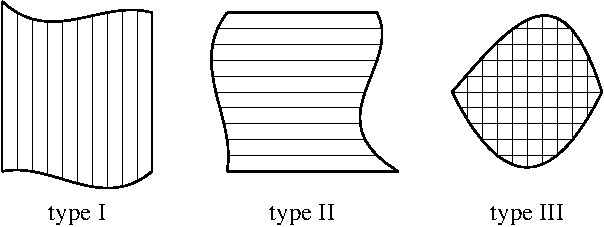
\includegraphics{figures/greenstypes}
\caption{Domain types for Green's theorem.\label{fig:greenstypes}}
\end{myfigureht}

%If we have a type I domain, then
%the paths given by the graphs of $f$ and $g$ together with the
%straight line segments between $g(a)$ and $f(a)$, and also between
%$g(b)$ and $f(b)$ give the boundary as a piecewise smooth path.  Similarly
%for type II, and hence for type II.  Therefore such domains are domains with
%piecewise smooth boundary.

%Let us state the version which we will prove.
We will only prove Green's theorem for type III domains.

%\begin{samepage}
%\begin{thm}[Green]
%Let $U \subset \R^2$ be a bounded domain with piecewise smooth boundary
%that is of type III.
%Suppose $P$ and $Q$ are continuously
%differentiable functions defined on some open set that contains the closure
%$\widebar{U}$ and suppose that $\partial U$ is positively oriented.  Then
%\begin{equation*}
%\int_{\partial U}
%P~ dx + Q~ dy
%=
%\int_{U}
%\left(\frac{\partial Q}{\partial x} - \frac{\partial P}{\partial y} \right)
%%~ dx ~ dy .
%.
%\end{equation*}
%\end{thm}
%\end{samepage}

\begin{proof}[Proof of Green's theorem for $U$ of type III]
Let $f,g,h,k$ be the functions defined above.
By \exerciseref{exercise:intovertypeIset},
$U$ is Jordan measurable and as $U$ is of type I, then
\begin{equation*}
\begin{split}
\int_U 
\left(- \frac{\partial P}{\partial y} \right)
& =
\int_a^b \int_{g(x)}^{f(x)}
\left(- \frac{\partial P}{\partial y} (x,y) \right)
~ dy ~ dx 
\\
& =
\int_a^b \Bigl(
- P\bigl(x,f(x)\bigr) +
P\bigl(x,g(x)\bigr)
\Bigr) ~ dx
\\
& =
\int_a^b P\bigl(x,g(x)\bigr) ~ dx 
-
\int_a^b P\bigl(x,f(x)\bigr) ~ dx .
\end{split}
\end{equation*}
We integrate $P~dx$ along the boundary.
The one-form $P~dx$ integrates to zero 
along the straight vertical lines in the boundary.  Therefore it is
only
integrated along the top and along the bottom.  As a parameter,
$x$ runs from left to right.  If we use the parametrizations that take $x$
to $\bigl(x,f(x)\bigr)$ and to
$\bigl(x,g(x)\bigr)$ we recognize path integrals above.  However the second
path integral is in the wrong direction; the top should be going right to
left, and so we must switch orientation.
\begin{equation*}
\int_{\partial U} P ~ dx
=
\int_a^b P\bigl(x,g(x)\bigr) ~ dx 
+
\int_b^a P\bigl(x,f(x)\bigr) ~ dx
=
\int_U 
\left(- \frac{\partial P}{\partial y} \right) .
\end{equation*}

Similarly, $U$ is also of type II.  The form $Q~dy$ integrates to zero along
horizontal lines.   So
\begin{equation*}
\int_U 
\frac{\partial Q}{\partial x}
=
\int_c^d \int_{k(y)}^{h(y)}
\frac{\partial Q}{\partial x}(x,y)
~ dx ~ dy 
=
\int_a^b \Bigl(
Q\bigl(y,h(y)\bigr) 
-
Q\bigl(y,k(y)\bigr)
\Bigr) ~ dx 
=
\int_{\partial U} Q ~ dy .
\end{equation*}
Putting the two together we obtain
\begin{equation*}
\int_{\partial U} P~ dx + Q ~ dy 
=
\int_{\partial U} P~ dx + \int_{\partial U} Q ~ dy 
=
\int_U 
\Bigl(-\frac{\partial P}{\partial y}\Bigr)
+
\int_U 
\frac{\partial Q}{\partial x}
=
\int_U 
\Bigl(
\frac{\partial Q}{\partial x}
-\frac{\partial P}{\partial y}
\Bigr) . \qedhere
\end{equation*}
\end{proof}

Let us illustrate the usefulness of Green's theorem on a fundamental result
about harmonic functions.

\begin{example}
Suppose $U \subset \R^2$ is an open set and
$f \colon U \to \R$ is harmonic, that is, $f$ is twice continuously
differentiable and
$\frac{\partial^2 f}{\partial x^2} +
\frac{\partial^2 f}{\partial y^2} = 0$.
We will prove one of the most fundamental properties of Harmonic functions.

Let $D_r = B(p,r)$ be closed disc such that its closure $C(p,r) \subset U$.  Write
$p = (x_0,y_0)$.  We orient
$\partial D_r$ positively.  See \exerciseref{green:balltype3orient}.
Then
\begin{equation*}
\begin{split}
0
& =
\frac{1}{2\pi r}
\int_{D_r}
\left(
\frac{\partial^2 f}{\partial x^2} +
\frac{\partial^2 f}{\partial y^2}
\right)
\\
& 
=
\frac{1}{2\pi r}
\int_{\partial D_r}
- \frac{\partial f}{\partial y} ~ dx + 
\frac{\partial f}{\partial x} ~ dy
\\
&
=
\frac{1}{2\pi r}
\int_0^{2\pi}
\biggl(
- \frac{\partial f}{\partial y} \bigl(x_0+r\cos(t),y_0+r\sin(t)\bigr) \bigl(-r\sin(t)\bigr)
\\
& \hspace{1.2in}
+ \frac{\partial f}{\partial x} \bigl(x_0+r\cos(t),y_0+r\sin(t)\bigr) r\cos(t)
\biggr) ~ dt
\\
&
=
\frac{d}{dr}
\left[
\frac{1}{2\pi}
\int_0^{2\pi}
f\bigl(x_0+r\cos(t),y_0+r\sin(t)\bigr) ~ dt
\right] .
\end{split}
\end{equation*}
Let $g(r) := 
\frac{1}{2\pi}
\int_0^{2\pi}
f\bigl(x_0+r\cos(t),y_0+r\sin(t)\bigr) ~ dt$.  Then $g'(r) = 0$ for all
$r > 0$.
The function is constant for $r >0$ and continuous at $r=0$ (exercise).
Therefore $g(0) = g(r)$ for all $r > 0$.  Therefore,
\begin{equation*}
g(r) = g(0) = 
\frac{1}{2\pi}
\int_0^{2\pi}
f\bigl(x_0+0\cos(t),y_0+0\sin(t)\bigr) ~ dt
=
f(x_0,y_0).
\end{equation*}
We
proved the \emph{\myindex{mean value property}} of harmonic functions:
\begin{equation*}
f(x_0,y_0) = 
\frac{1}{2\pi}
\int_0^{2\pi}
f\bigl(x_0+r\cos(t),y_0+r\sin(t)\bigr) ~ dt 
=
\frac{1}{2\pi r}
\int_{\partial D_r} f ~ ds .
\end{equation*}
That is, the value at $p = (x_0,y_0)$ is the average over a circle of any
radius $r$ centered at $(x_0,y_0)$.
\end{example}

\subsection{Exercises}

\begin{exercise} \label{green:balltype3orient}
Prove that a disc $B(p,r) \subset \R^2$ is a type III domain, and prove that
the orientation given by the parametrization $\gamma(t) =
\bigl(x_0+r\cos(t),y_0+r\sin(t)\bigr)$ where $p = (x_0,y_0)$ is the positive
orientation of the boundary $\partial B(p,r)$.
\end{exercise}

\begin{exercise}
Prove that any bounded domain with piecewise smooth boundary that is
convex is a type III domain.
\end{exercise}

\begin{exercise}
Suppose $V \subset \R^2$ is a domain with piecewise smooth boundary that is
a type III domain and suppose that $U \subset \R^2$ is a domain such that
$\widebar{V} \subset U$.  Suppose $f \colon U \to \R$ is a twice
continuously differentiable function.  Prove that
$\int_{\partial V}
\frac{\partial f}{\partial x} dx + 
\frac{\partial f}{\partial y} dy = 0$.
\end{exercise}

\begin{samepage}
\begin{exercise}
For a disc $B(p,r) \subset \R^2$, orient the boundary $\partial B(p,r)$
positively:
\begin{enumerate}[a)]
\item
Compute $\displaystyle \int_{\partial B(p,r)} -y ~ dx$.
\item
Compute $\displaystyle \int_{\partial B(p,r)} x ~ dy$.
\item
Compute $\displaystyle \int_{\partial B(p,r)} \frac{-y}{2} ~ dy +
\frac{x}{2} ~ dy$.
\end{enumerate}
\end{exercise}
\end{samepage}

\begin{exercise}
Using Green's theorem show that the area of a triangle with
vertices
$(x_1,y_1)$,
$(x_2,y_2)$,
$(x_3,y_3)$ is
$\frac{1}{2}\sabs{x_1y_2 + x_2 y_3 + x_3 y_1 - y_1x_2 - y_2x_3 - y_3x_1}$.
Hint: see previous exercise.
\end{exercise}

\begin{exercise}
Using the mean value property prove the \emph{\myindex{maximum principle}} for harmonic
functions:
Suppose $U \subset \R^2$ is a connected open set and
$f \colon U \to \R$ is harmonic. Prove that
if $f$ attains a maximum at $p \in U$, then $f$ is constant.
\end{exercise}

\begin{exercise}
Let $f(x,y) := \ln \sqrt{x^2+y^2}$.
\begin{enumerate}[a)]
\item
Show $f$ is harmonic where defined.
\item
Show $\lim_{(x,y) \to 0} f(x,y) = -\infty$.
\item
Using a circle $C_r$ of radius
$r$ around the origin, compute $\frac{1}{2\pi r} \int_{\partial C_r} f ds$.
What happens as $r \to 0$?
\item
Why can't you use Green's theorem?
\end{enumerate}
\end{exercise}


